\section{ANEXOS}
\subsection*{ANEXO A: Explicación de los hiperparámetros y resultados de YOLO}
\label{subsec:A}

Las redes neuronales como \texttt{YOLO} y en general todas las que utilizan entrenamiento supervisado, tienen como objetivo acercarse lo máximo posible al resultado esperado en las etiquetas de entrenamiento. 
A lo largo de este entrenamiento se van actualizando parámetros (valores que sí cambian en entrenamiento) como son los pesos, los \texttt{bias} y otros elementos. Esta búsqueda de aproximación se puede ver 
reflejada como la búsqueda de mínimos globales en una función, en la mayoría de casos es buscar los mínimos globales de la función de perdidas. Esto se puede ver en la \autoref{fig:GradientDescendGlobales}.

\begin{figure}[H]
    \centering
    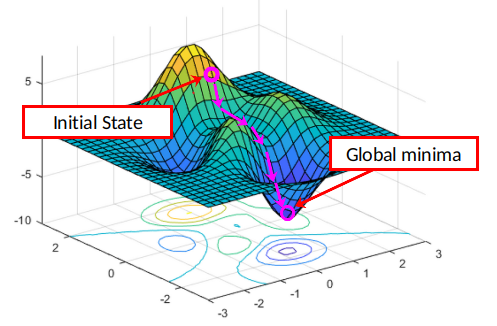
\includegraphics[width=0.5\textwidth]{images/13/a/GradientDescend.png}
    \caption{Búsqueda de mínimos globales por un algoritmo de aprendizaje automático\cite{doleronDeepLearningScratch2023}}
    \label{fig:GradientDescendGlobales}
\end{figure}

Los modelos de \texttt{YOLO} tienen definidos una serie de hiperparámetros (valores que no cambian en entrenamiento) que sirven como ajustes fijos durante en el entrenamiento. 
Estos hiperparámetros ajustan la manera en la que el algoritmo decide el siguiente paso a tomar en su búsqueda de un mínimo global y pueden acelerar o ralentizar el tiempo necesario 
de entrenamiento para alcanzar unos valores de perdida adecuados. Algunos de los hiperparámetros más típicos\cite{ultralyticsConfiguration} son:

\begin{itemize}
    \item \textbf{Learning Rate inicial}: es el valor que afecta cuanto se cambian los pesos entre época. Por defecto es \texttt{0.01}, que puede parecer poco, pero es mejor dar pasos pequeños para llegar al mínimo global.
    \item \textbf{Learning Rate final}: es una fracción del valor inicial. Según se realiza el entrenamiento de la red es normal reducir el \texttt{Learning Rate} para ajustar de forma más fina. Por defecto es \texttt{0.01}.
    \item \textbf{Momentum}: es una variable que permite tener en cuenta que camino se ha recorrido en la anterior época, para no volver a situaciones anteriores y seguir progresando. Por defecto es \texttt{0.937}.
    \item \textbf{Weight Decay}: hiperparámetro para prevenir sobreajuste y penalizar los pesos que son extremadamente grandes en la red.
    \item \textbf{Épocas de calentamiento}: número de épocas que se utilizaran para ir poco a poco acercándose a los valores iniciales de \texttt{Learning Rate}. Por defecto su valor es 3.
    \item \textbf{Tamaño de lote}: número de imágenes que se utilizaran en una pasada. Si tenemos 50 imágenes y el tamaño del lote es 10, se pasaran 10 y se ajustaran los pesos, y en este caso una época se compondra 
    de 5 pasadas de lote.
    \item \textbf{Número de épocas}
    \item \textbf{Número de capas ocultas}
\end{itemize}
\clearpage
Además, \texttt{YOLO} utiliza de base una herramienta de aumento de datos simple, por lo tanto tenemos muchos hiperparámetros para ajustar su funcionamiento:

\begin{itemize}
    \item \textbf{Hsv componente h}: ajusta el \texttt{Hue} de la imagen por una fracción que por defecto es \texttt{0.015}.
    \item \textbf{Hsv componente s}: ajusta la saturación de la imagen por una fracción que por defecto es \texttt{0.7}, permite simular diferentes condiciones de iluminación.
    \item \textbf{Hsv componente v}: modifica el brilo de la imagen, por defecto a una fracción de \texttt{0.4}.
    \item \textbf{Translate}: mueve la imagen horizontal y verticalmente por defecto un \texttt{10\%}.
    \item \textbf{Scale}: ajusta el tamaño de la imagen para simular diferentes distancias a la cámara. Por defecto \texttt{0.5}.
    \item \textbf{Fliplr}: espeja la imagen horizontalmente con una probabilidad por defecto de \texttt{0.5}.
    \item \textbf{Mosaic}: permite combinar 4 imágenes en una para crear imágenes compuestas que mejoran mucho la calidad del entrenamiento. Por defecto siempre está activo.
    \item \textbf{Erasing}: borra partes de la imagen de forma aleatoria para que el modelo sepa reconocer segmentos del elemento y que sea capaz de detectar características más específicas.
    \item \textbf{Crop fraction}: de forma aleatoria corta la imagen a fracciones de su tamaño original.
\end{itemize}
El resultado de este aumento de datos se puede ver en los lotes con los que se entrena la red como el de la \autoref{fig:AumentoDatosYolo}, donde vemos cambios de brillo, saturación, recortes de imagen y 
combinación de imágenes en diferentes tamaños.
\begin{figure}[H]
    \centering
    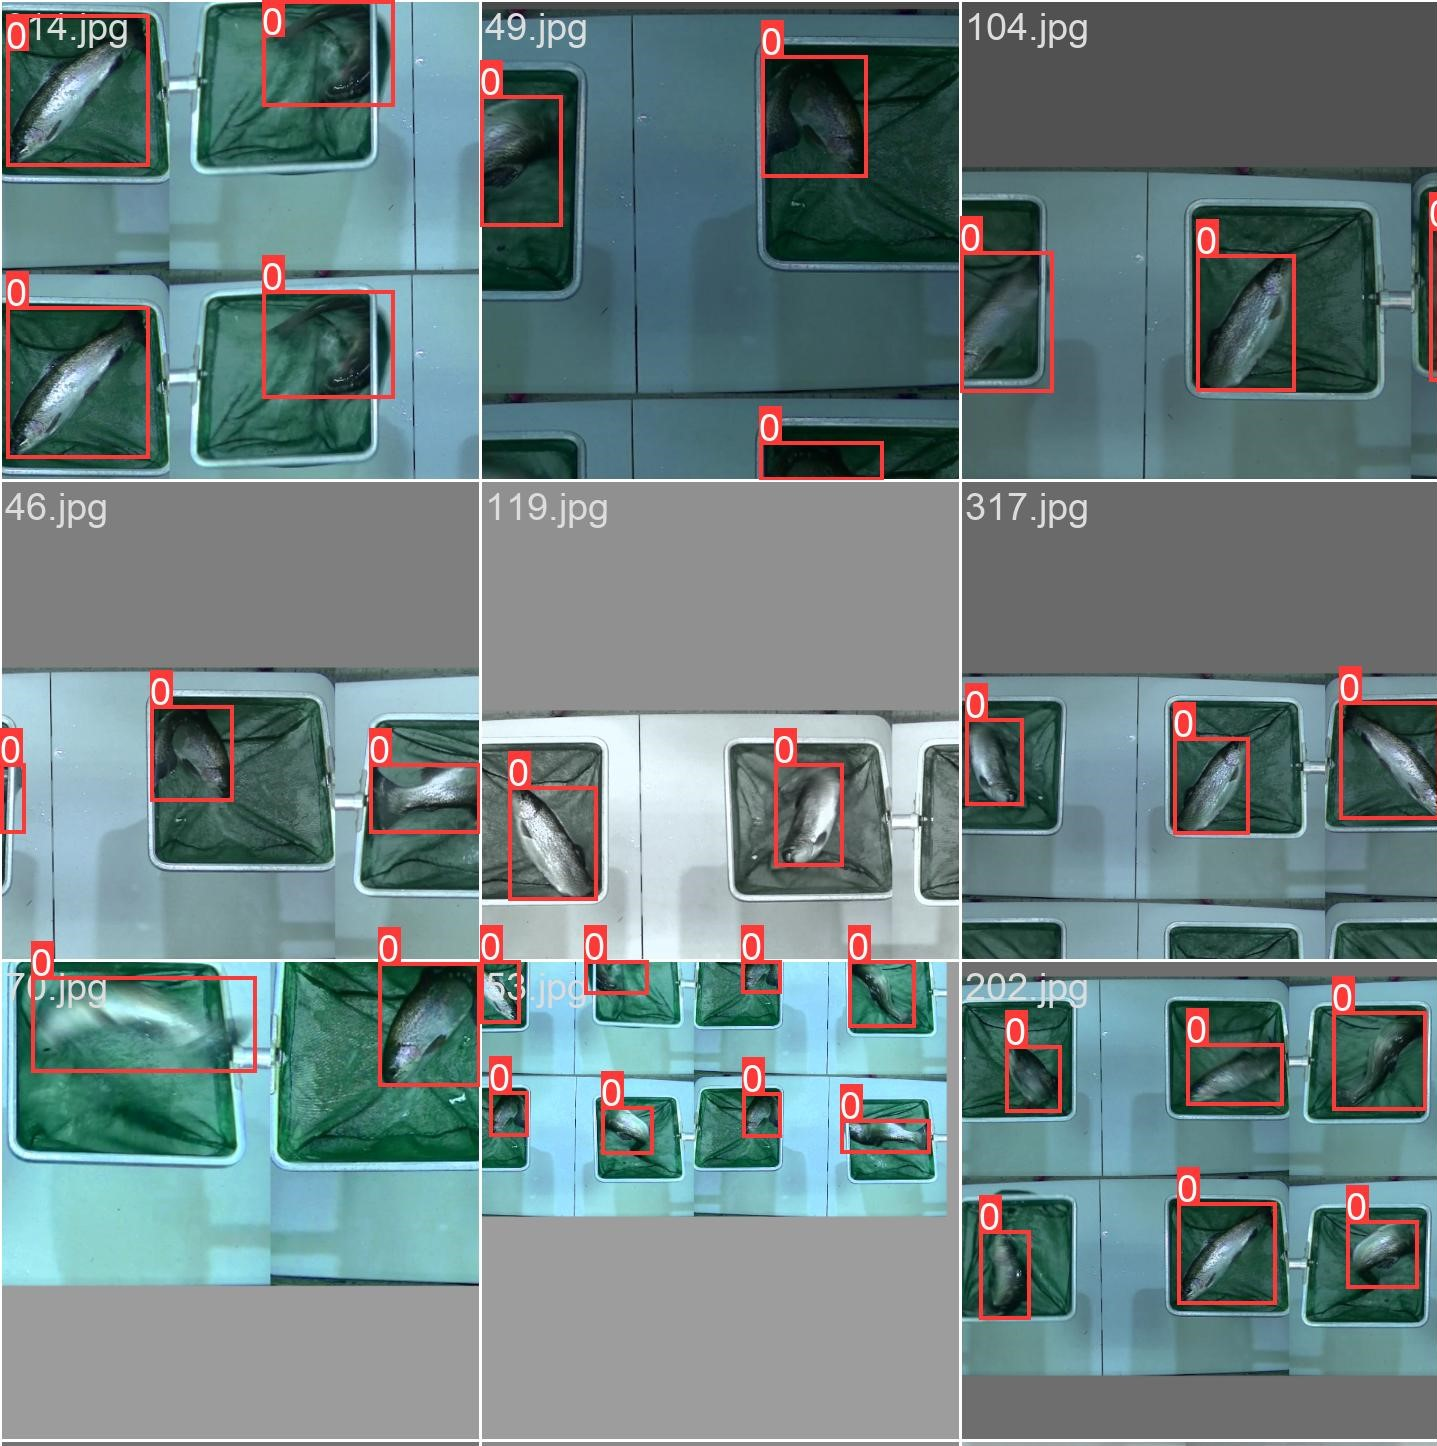
\includegraphics[width=0.7\textwidth]{images/13/a/EjemploAumento.jpg}
    \caption{Ejemplo de aumento de datos automático de \texttt{YOLO}}
    \label{fig:AumentoDatosYolo}
\end{figure}
\clearpage
\subsection*{ANEXO B: Datos de entrenamiento}
\label{subsec:B}
\subsubsection*{Entrenamiento 1}
\label{train:1}
\begin{itemize}
    \item \textbf{Fecha}: 9 de abril de 2024 (Prueba de concepto).
    \item \textbf{Descripción del conjunto de datos}: 24 imágenes seleccionadas manualmente del video \verb|23_NT_R1_J1_P1_2.mp4|. Conjunto dividido en 70-15-15 para los respectivos subconjuntos.
    \item \textbf{Resultados de entrenamiento}: En las siguientes figuras se observan  unos resultados que aparentan buenos  para ser un primer entrenamiento, pero debido al conjunto de datos con datos similares entre sí, en 
    situaciones de posiciones de trucha nuevas, se observó problemas en la precisión de la red. Aparte de esto se puede ajustar más, ya que con 100 épocas vemos que se para cuando todavía hay una tendencia 
    descendente en el error en el conjunto de validación.
    
    \begin{figure}[H]
        \centering
        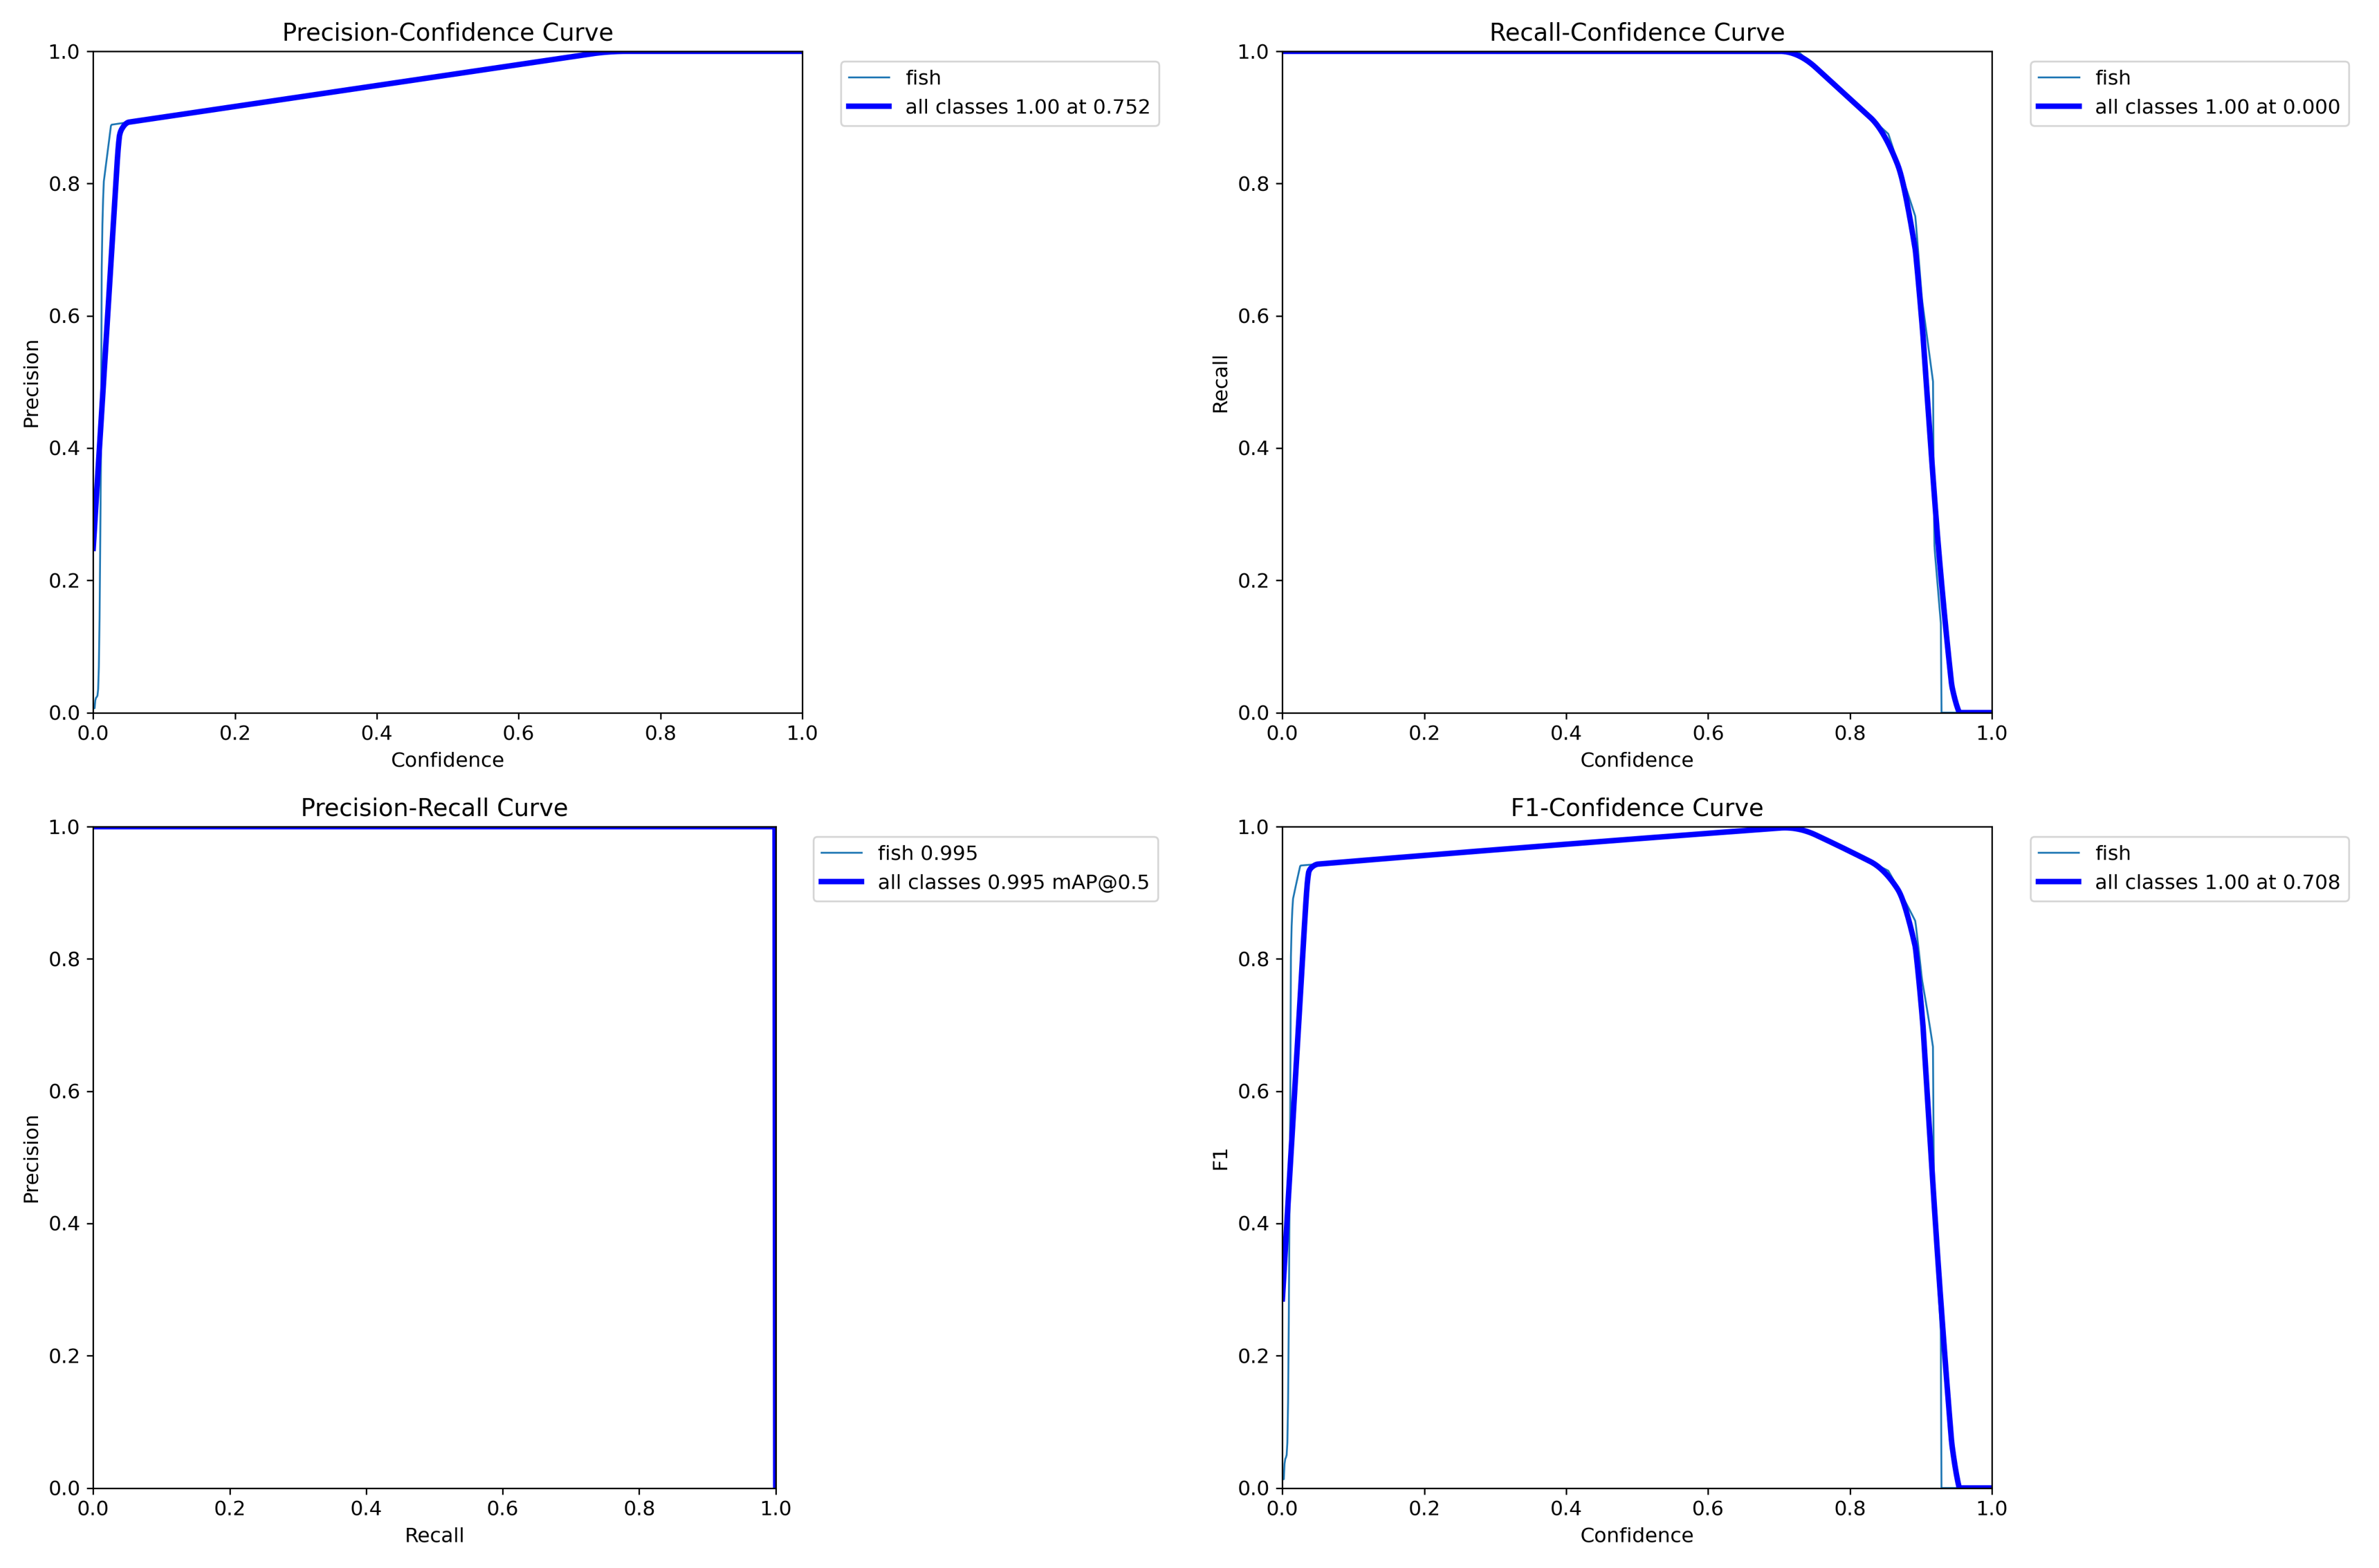
\includegraphics[width=0.9\textwidth]{images/13/b/1/PR.png}
        \caption{Gráficas de estadísticos finales del entrenamiento 1}
        \label{fig:Estadisticos1}
    \end{figure}
    \begin{figure}[H]
        \centering
        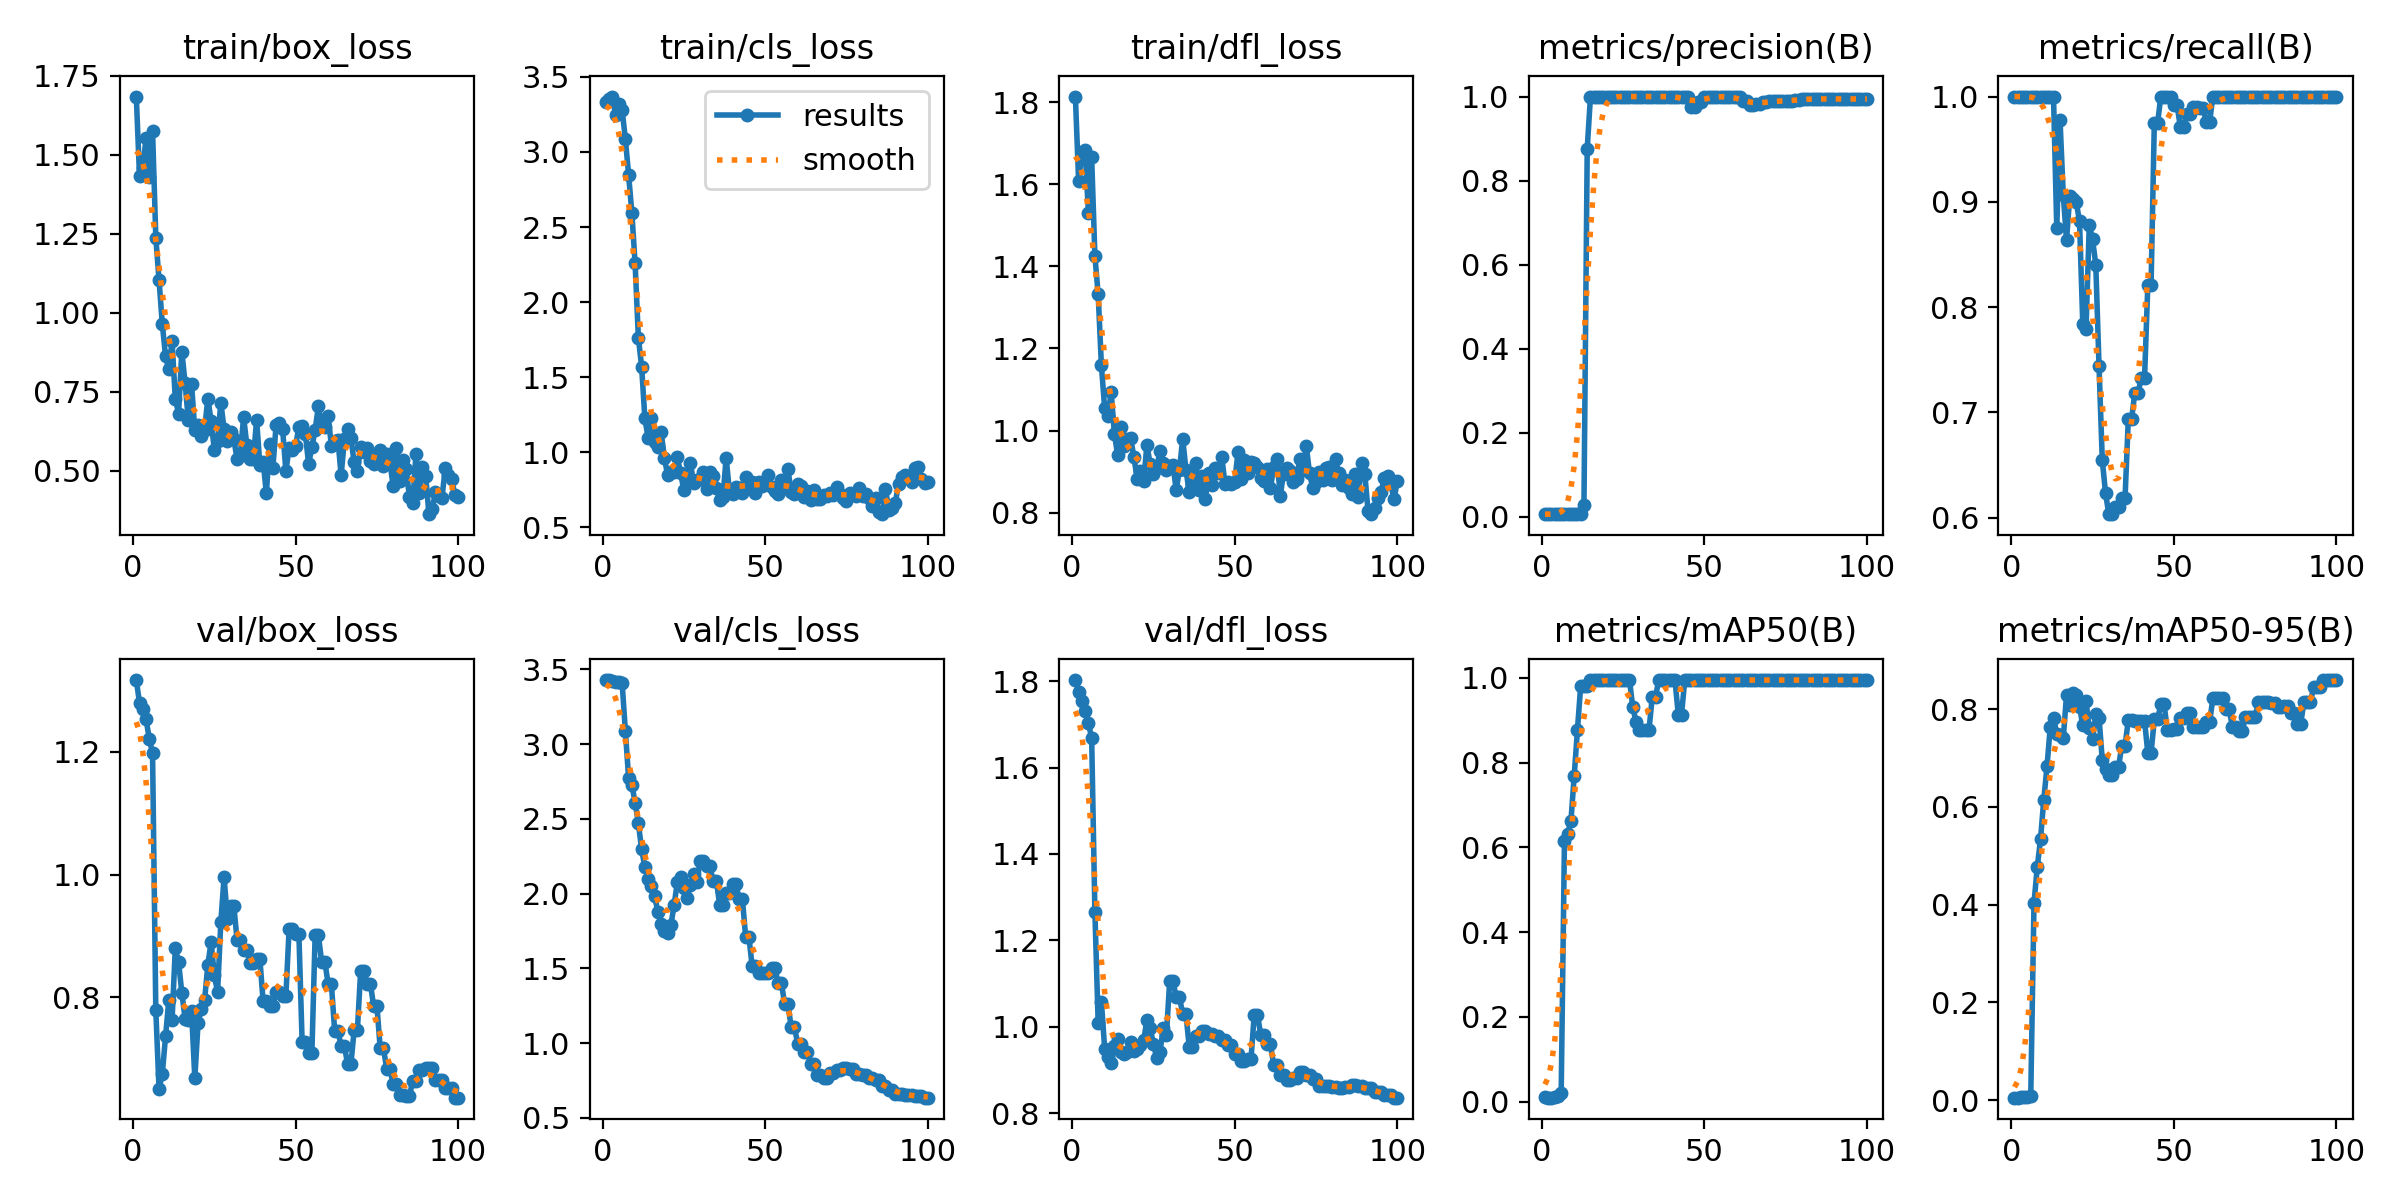
\includegraphics[width=0.9\textwidth]{images/13/b/1/results.png}
        \caption{Gráficas de evolución en épocas del entrenamiento 1}
        \label{fig:Resultados1}
    \end{figure}
\end{itemize}
\subsubsection*{Entrenamiento 2}
\label{train:2}
\begin{itemize}
    \item \textbf{Fecha}: 25 de abril de 2024.
    \item \textbf{Descripción del conjunto de datos}: al conjunto del \hyperref[train:1]{entrenamiento de prueba} se le añadieron imágenes extra y situaciones con redes vacías. En total 50 imágenes en división 70-15-15 para los subconjuntos.
    \item \textbf{Resultados del entrenamiento}: A través del aumento de datos del conjunto y con el mismo número de épocas, se puede observar en la \autoref{fig:Estadisticos2} que hemos mejorado mucho el \texttt{recall} teniendo menos falsos positivos, 
    pero hemos perdido precisión en situaciones de poca confianza, esto puede ser debido al añadir imágenes de redes sin peces, pero no es nada problemático, ya que para \texttt{Bounding Boxes} con tan poca confianza, es mejor no procesarlas. 
    Aparte se ve en la \autoref{fig:Resultados2} que hemos mejorado mucho la precisión en la perdida de las \texttt{Bounding Boxes}, esto era el objetivo. Vemos que el resto de parametros no han cambiado mucho, buena señal.
    \begin{figure}[H]
        \centering
        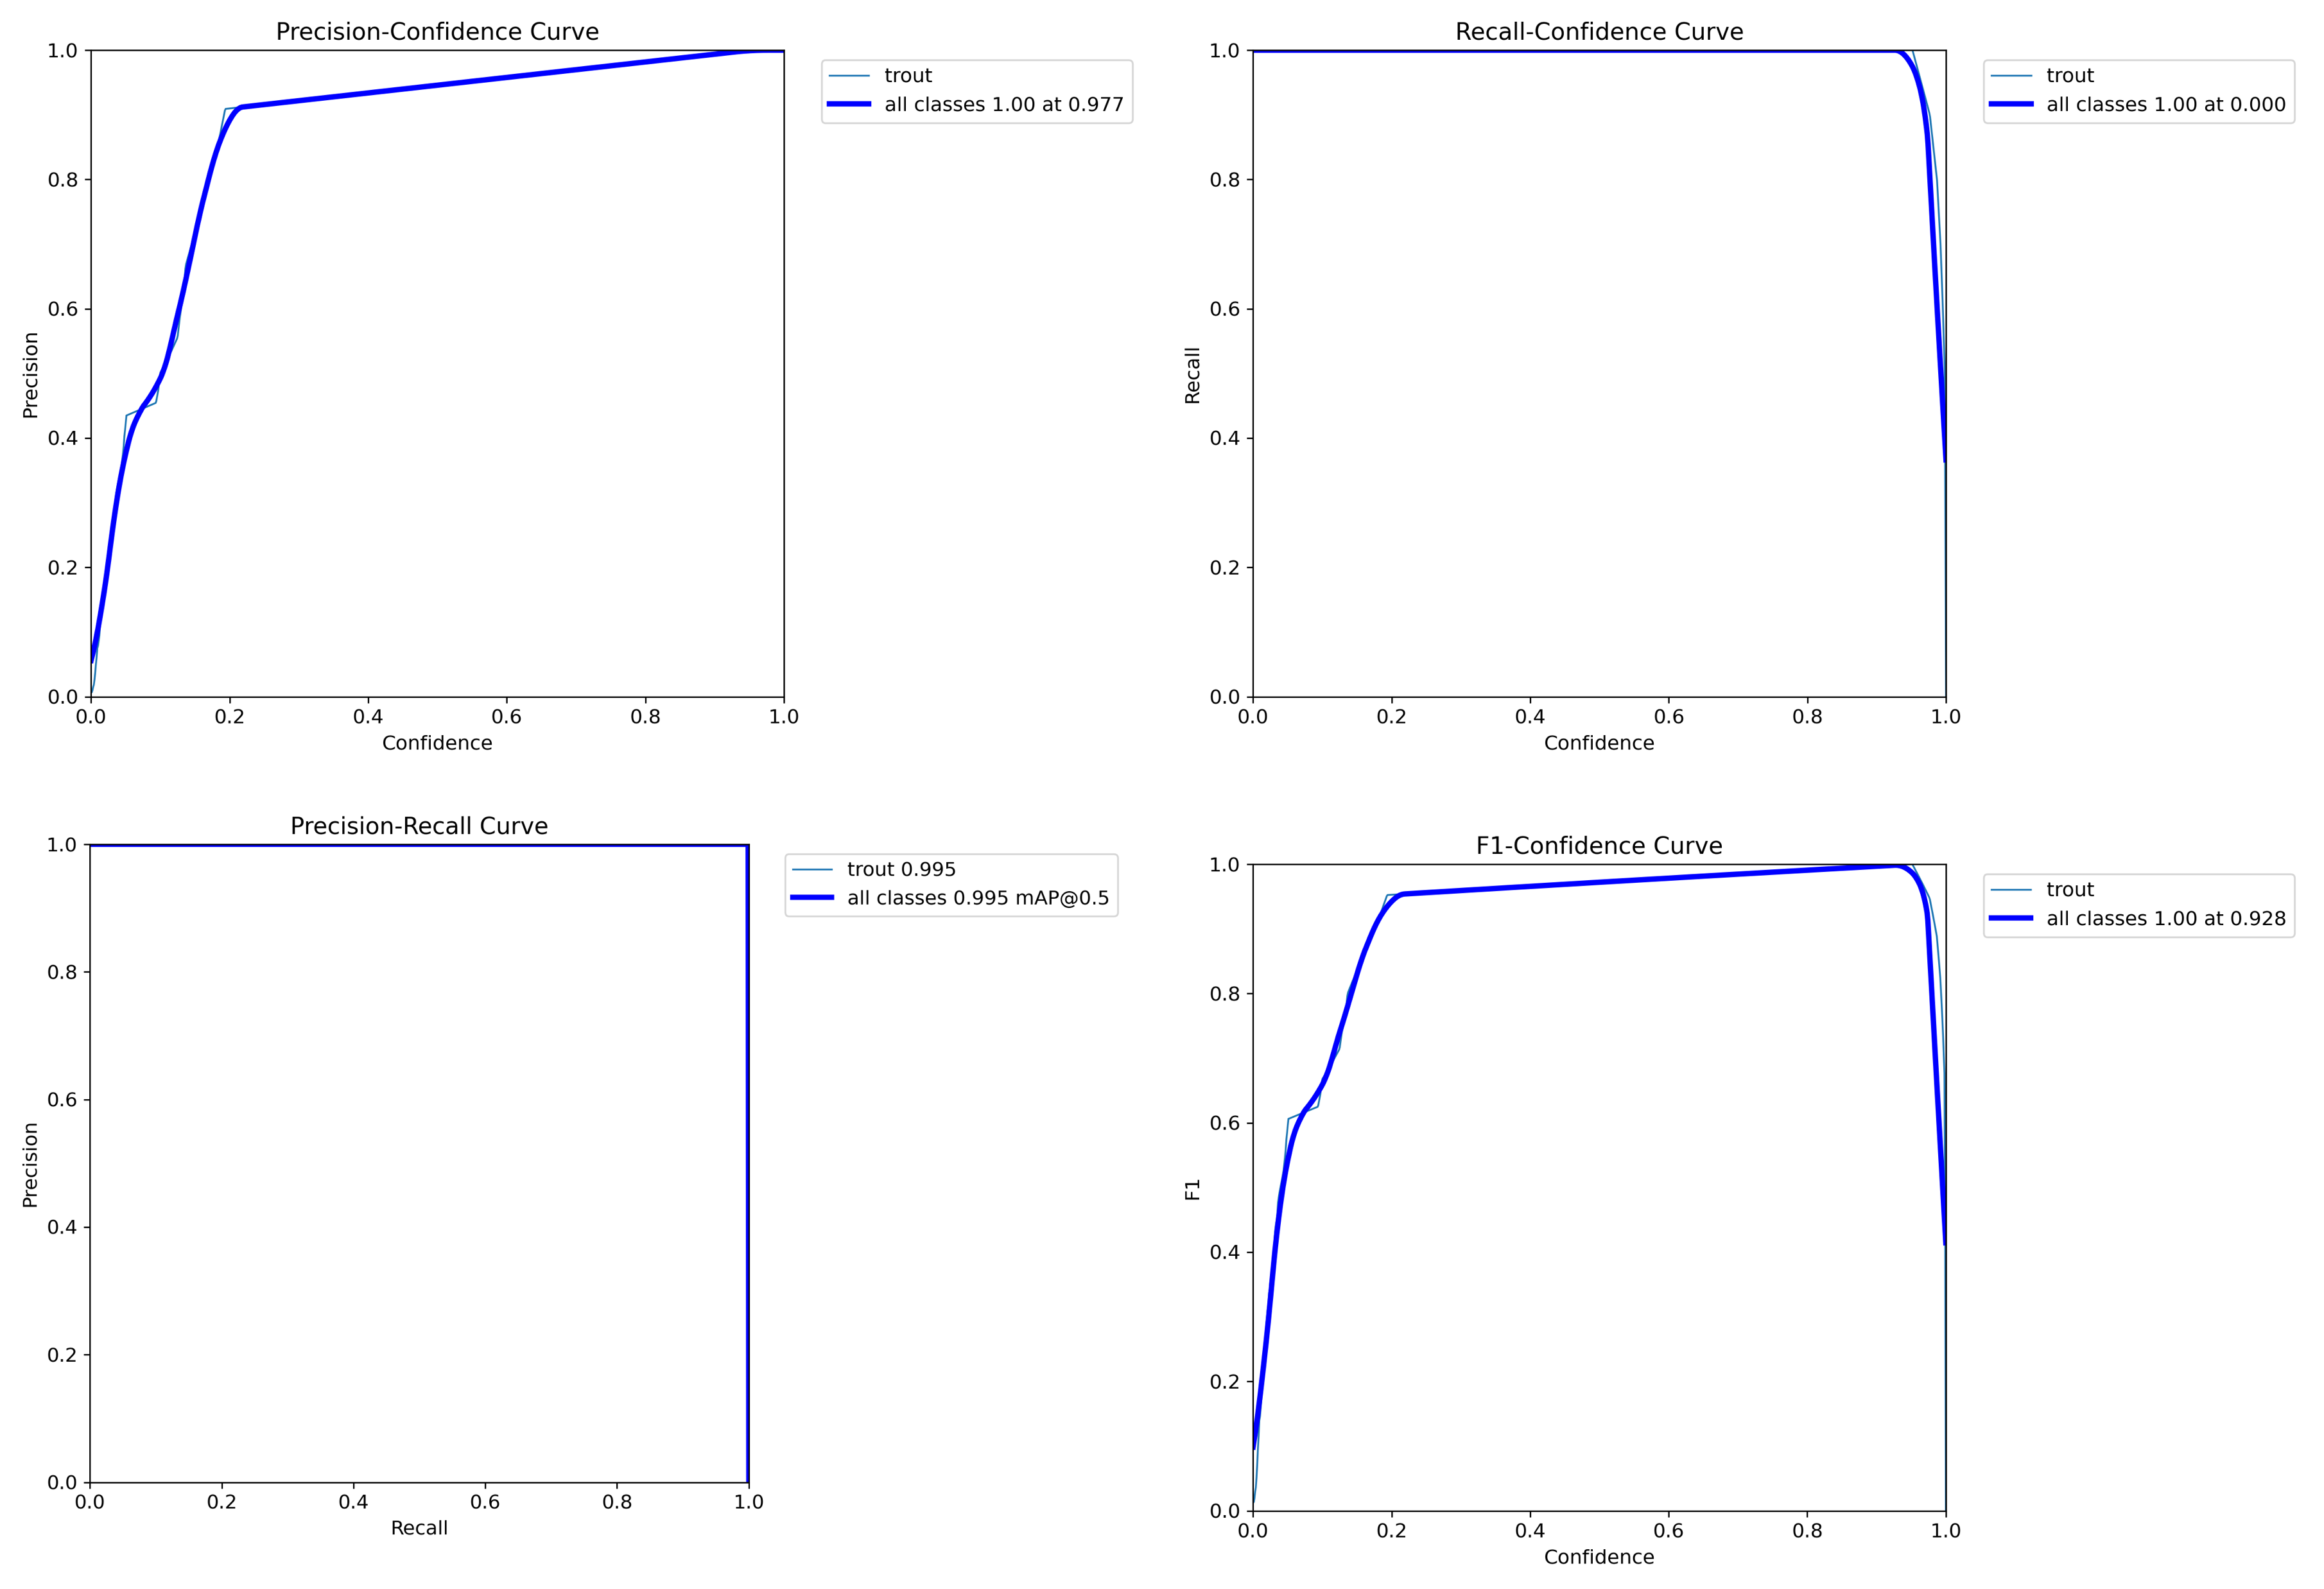
\includegraphics[width=0.82\textwidth]{images/13/b/2/graficas2.png}
        \caption{Gráficas de estadísticos finales del entrenamiento 2}
        \label{fig:Estadisticos2}
    \end{figure}
    \begin{figure}[H]
        \centering
        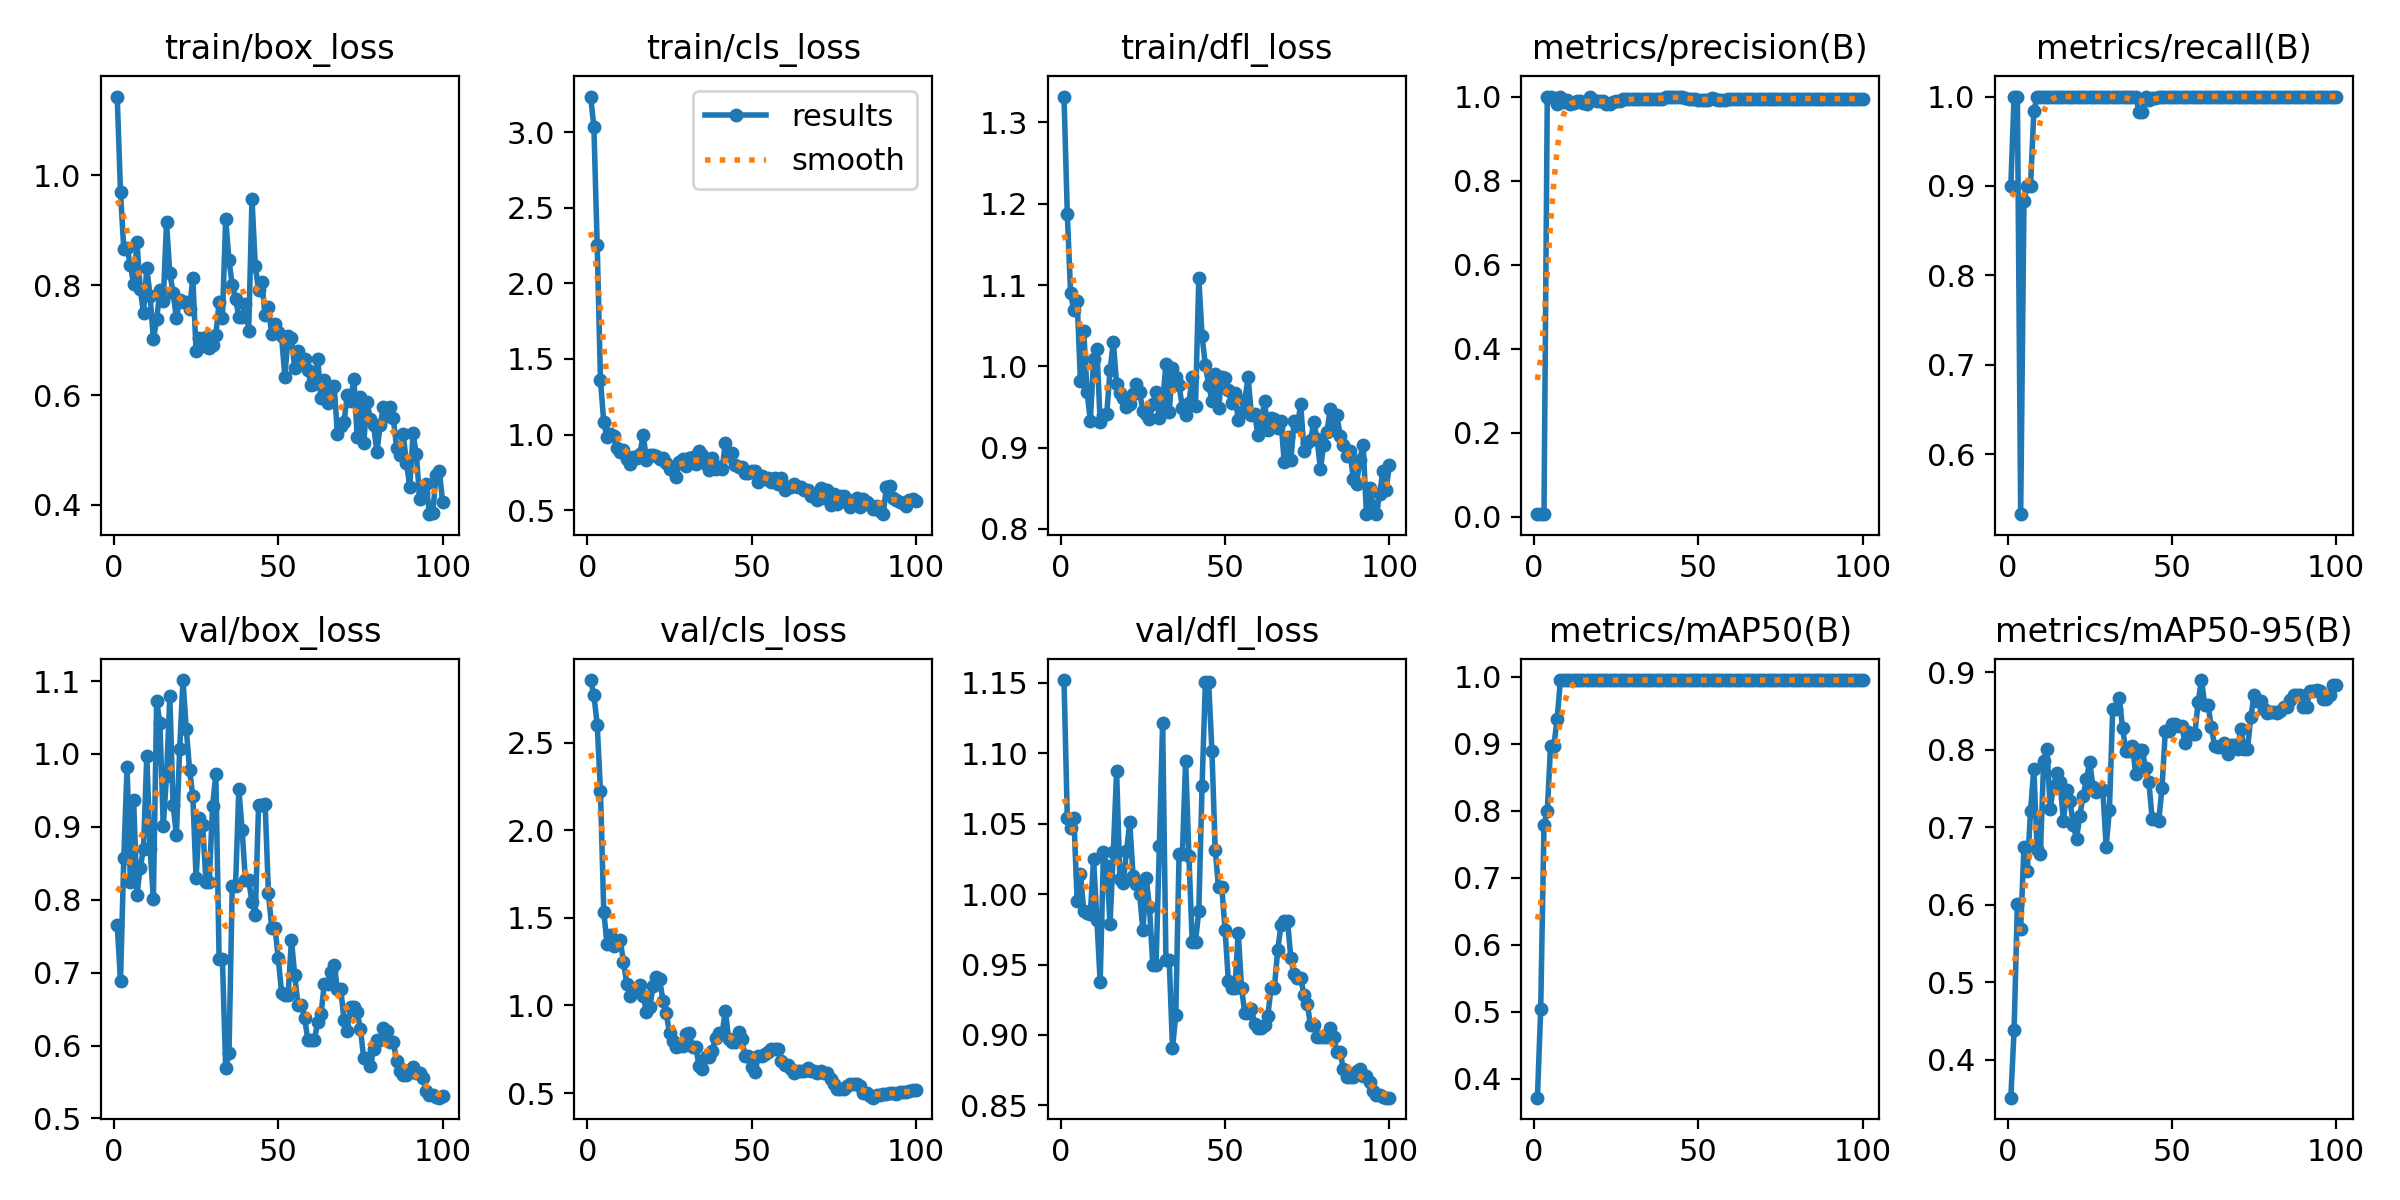
\includegraphics[width=0.9\textwidth]{images/13/b/2/results.png}
        \caption{Gráficas de evolución en épocas del entrenamiento 2}
        \label{fig:Resultados2}
    \end{figure}
\end{itemize}
\subsubsection*{Entrenamiento 3}
\label{train:3}
\begin{itemize}
    \item \textbf{Fecha}: 4 de mayo de 2024.
    \item \textbf{Descripción del conjunto de datos}: Mismo conjunto que el \hyperref[train:2]{entrenamiento anterior}.
    \item \textbf{Resultados del entrenamiento}: a través del aumento de las épocas hasta 300, se pudo observar como se podían alcanzar valores de error en las \texttt{Bounding Boxes} bastante más bajas. 
    Este entrenamiento también dejo claro que el conjunto de datos de validación era demasiado reducido y no era suficientemente representativo, las imágenes eran muy similares entre sí.

    \begin{figure}[H]
        \centering
        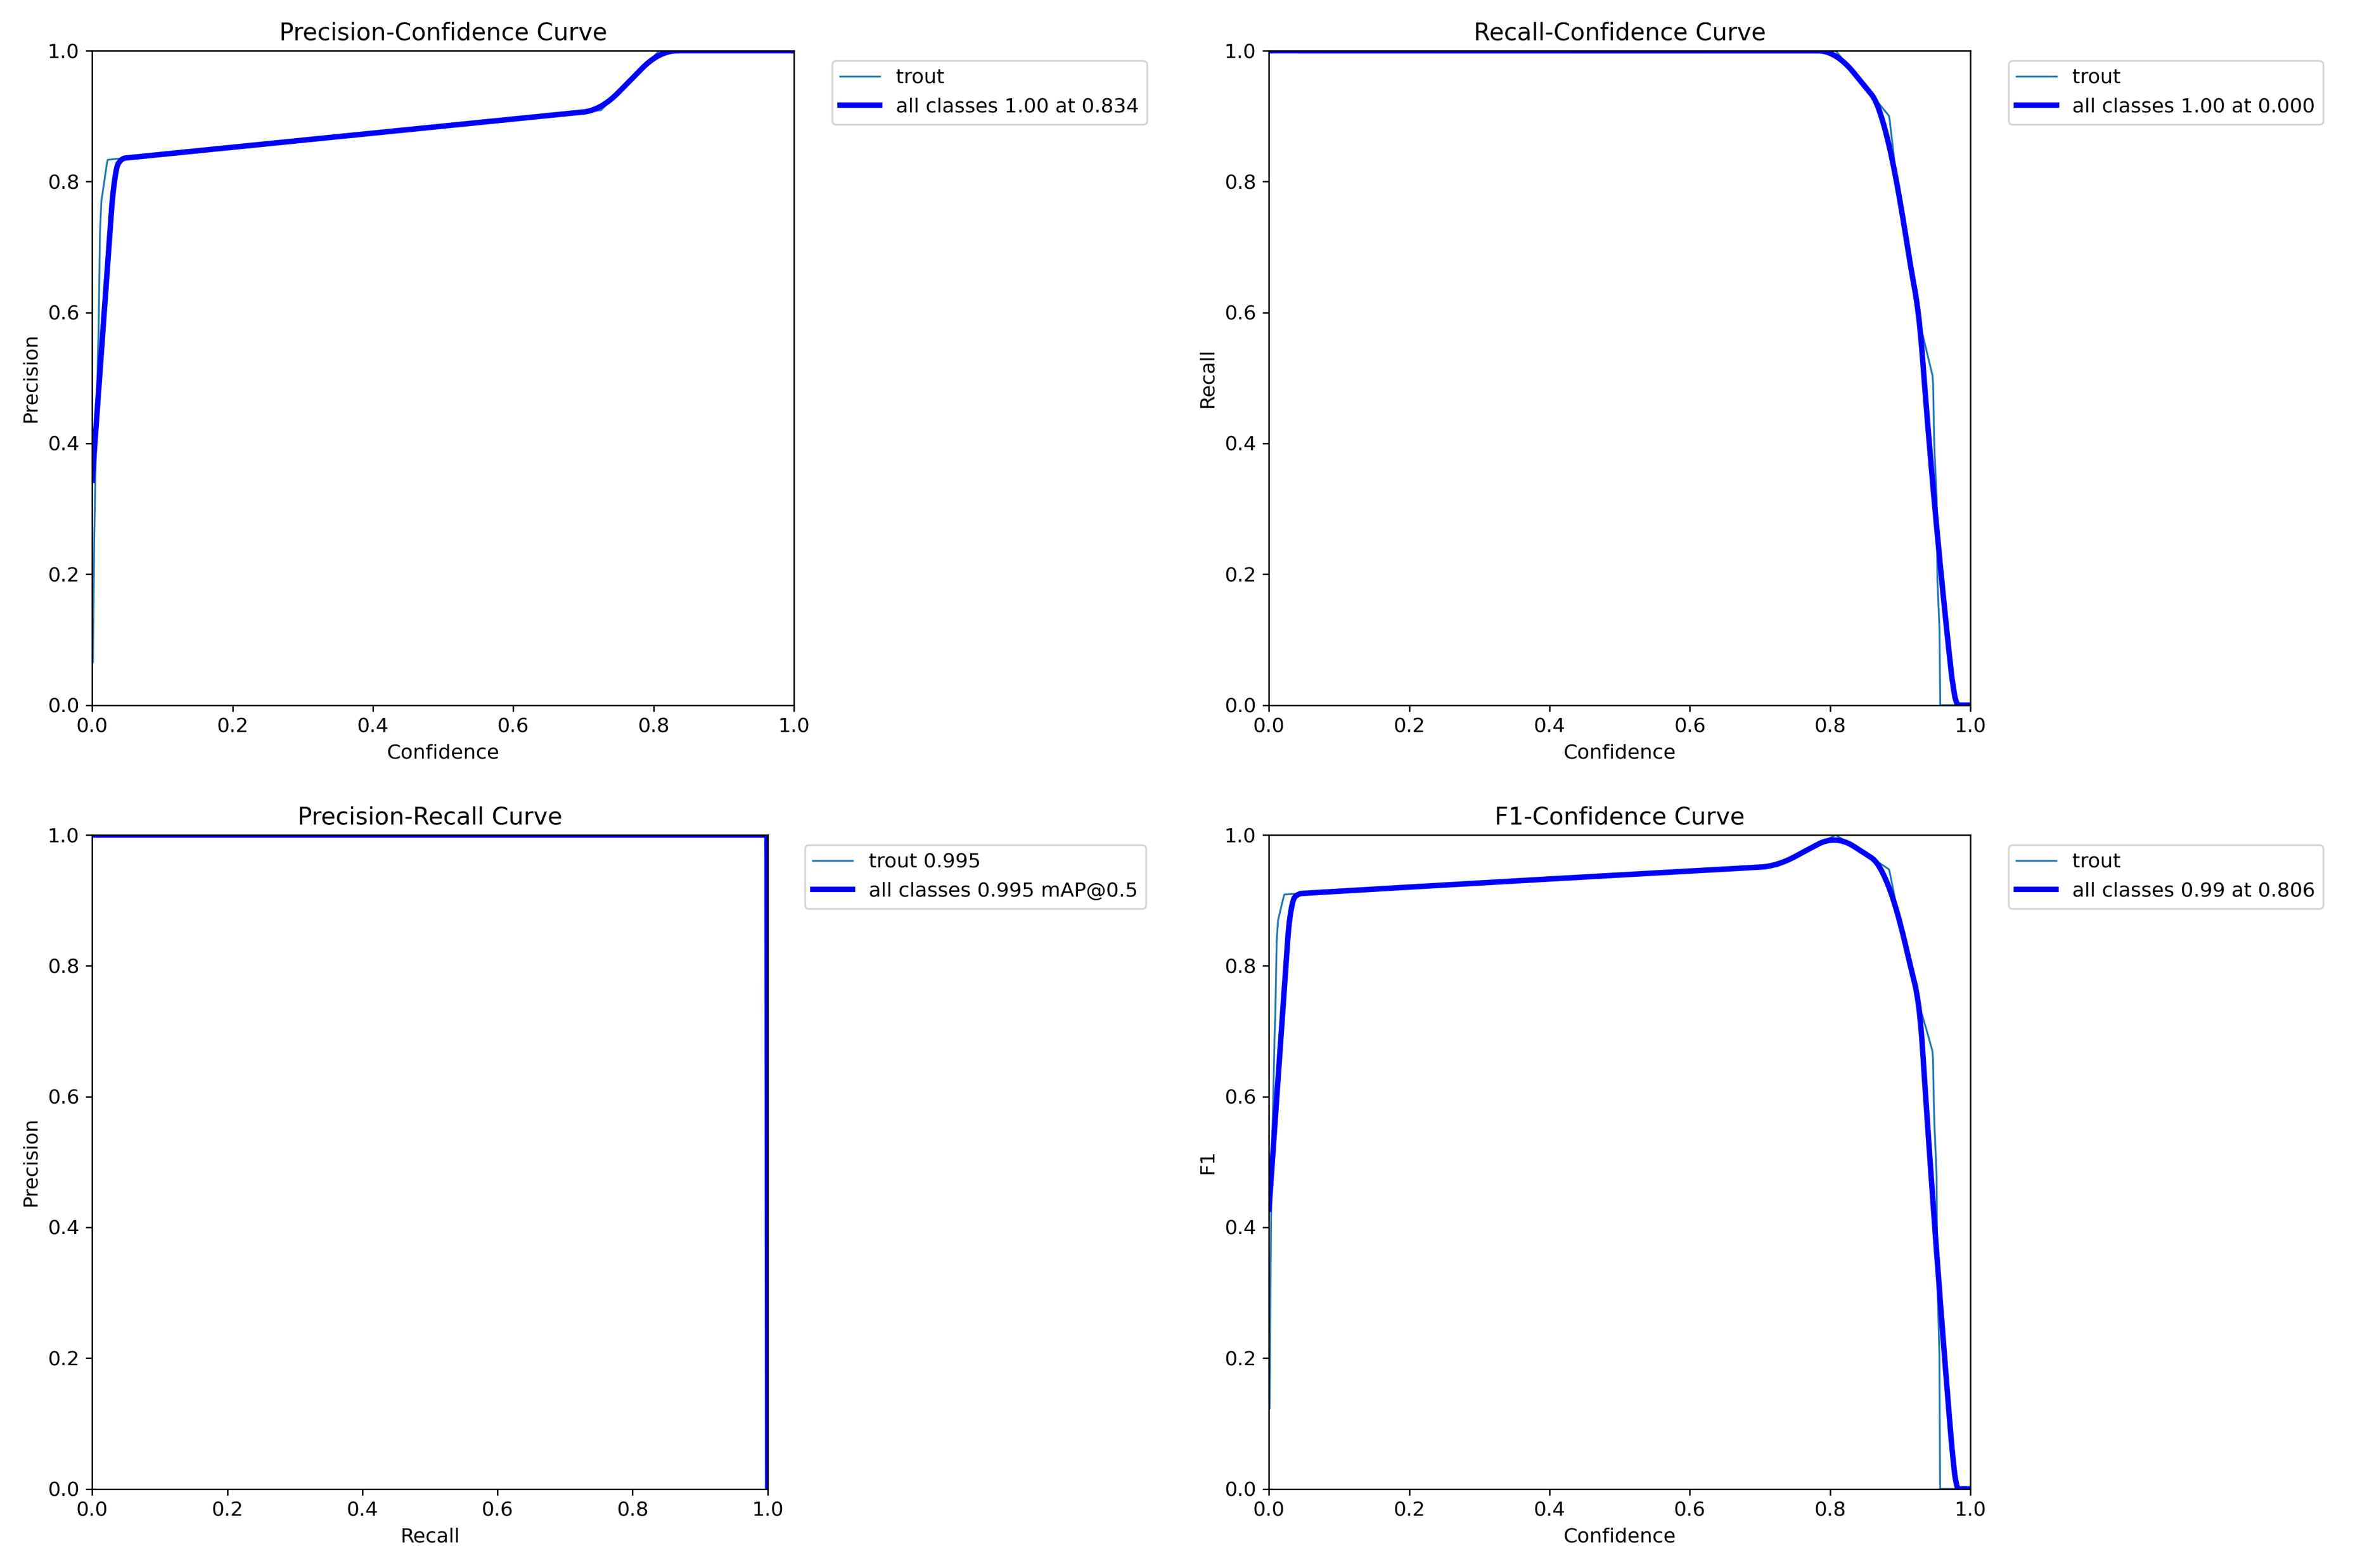
\includegraphics[width=0.95\textwidth]{images/13/b/3/graficas2.png}
        \caption{Gráficas de estadísticos finales del entrenamiento 3}
        \label{fig:Estadisticos3}
    \end{figure}
    \begin{figure}[H]
        \centering
        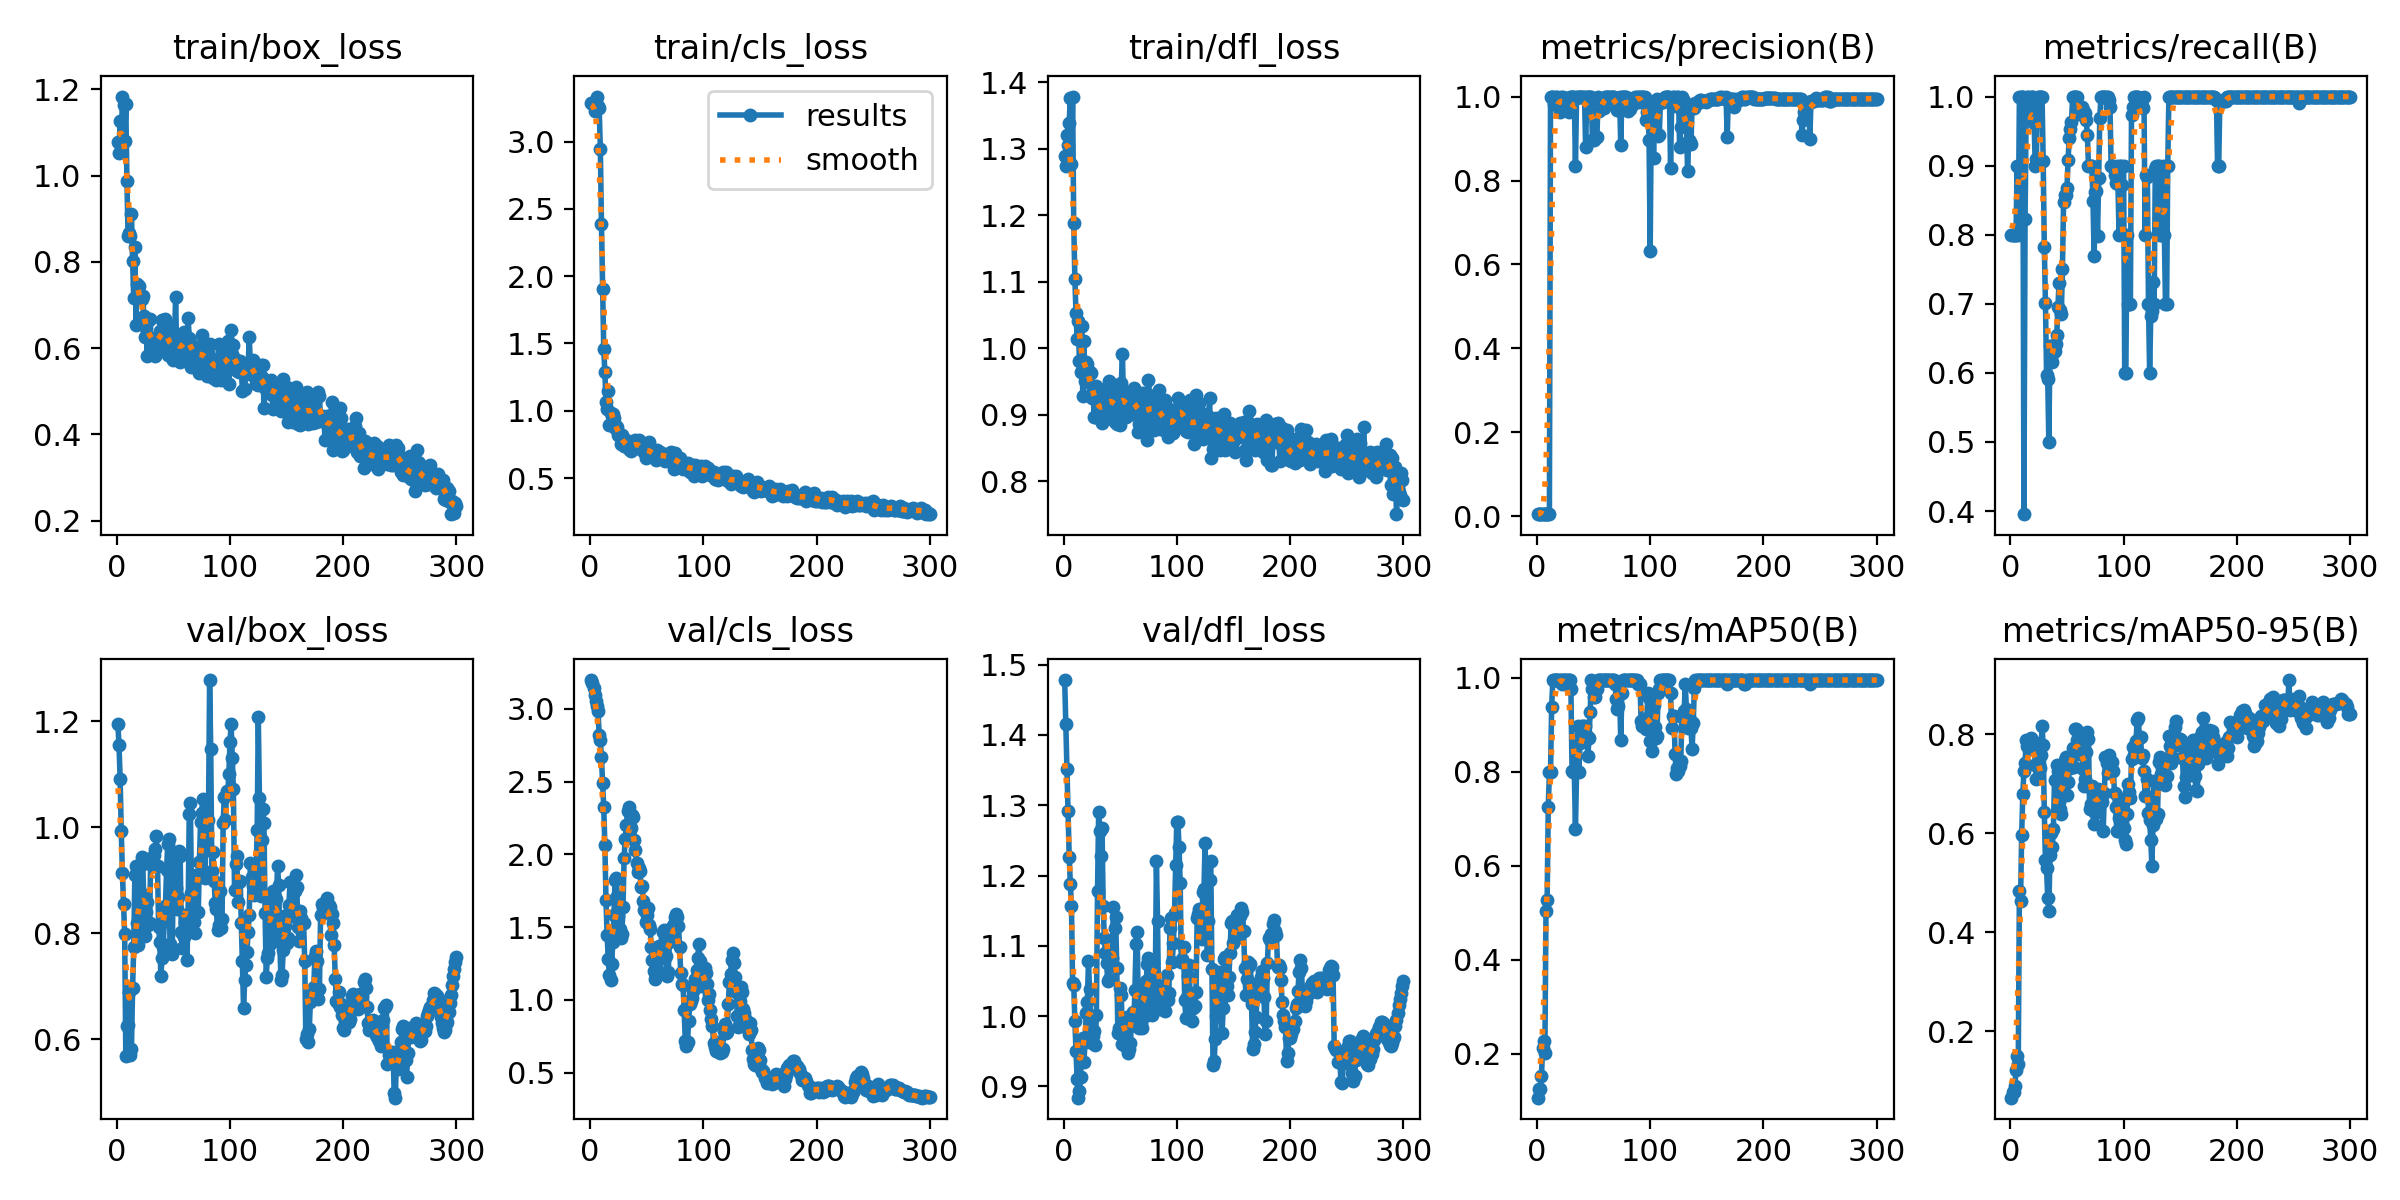
\includegraphics[width=0.95\textwidth]{images/13/b/3/results.png}
        \caption{Gráficas de evolución en épocas del entrenamiento 3}
        \label{fig:Resultados3}
    \end{figure}
\end{itemize}
\clearpage
\subsubsection*{Entrenamiento 4}
\label{train:4}
\begin{itemize}
    \item \textbf{Fecha}: 4 de mayo de 2024.
    \item \textbf{Descripción del conjunto de datos}: el conjunto de datos fue expandido con imágenes de los videos antiguos, obteniendo en total 84 imágenes representativas divididas en 70-15-15.
    \item \textbf{Resultados del entrenamiento}: por los nuevos tipos de imágenes añadidas, hemos perdido en la mayoría de métricas, pero esta red es mucho más representativa para los datos reales. 
    Además de esto, el conjunto de validación que se usa de referencia ahora es mucho más realista y tiene imágenes difíciles que implican movimientos, ya que para imágenes de truchas estáticas ha 
    estado funcionando correctamente durante todos los entrenamientos.
    
    \begin{figure}[H]
        \centering
        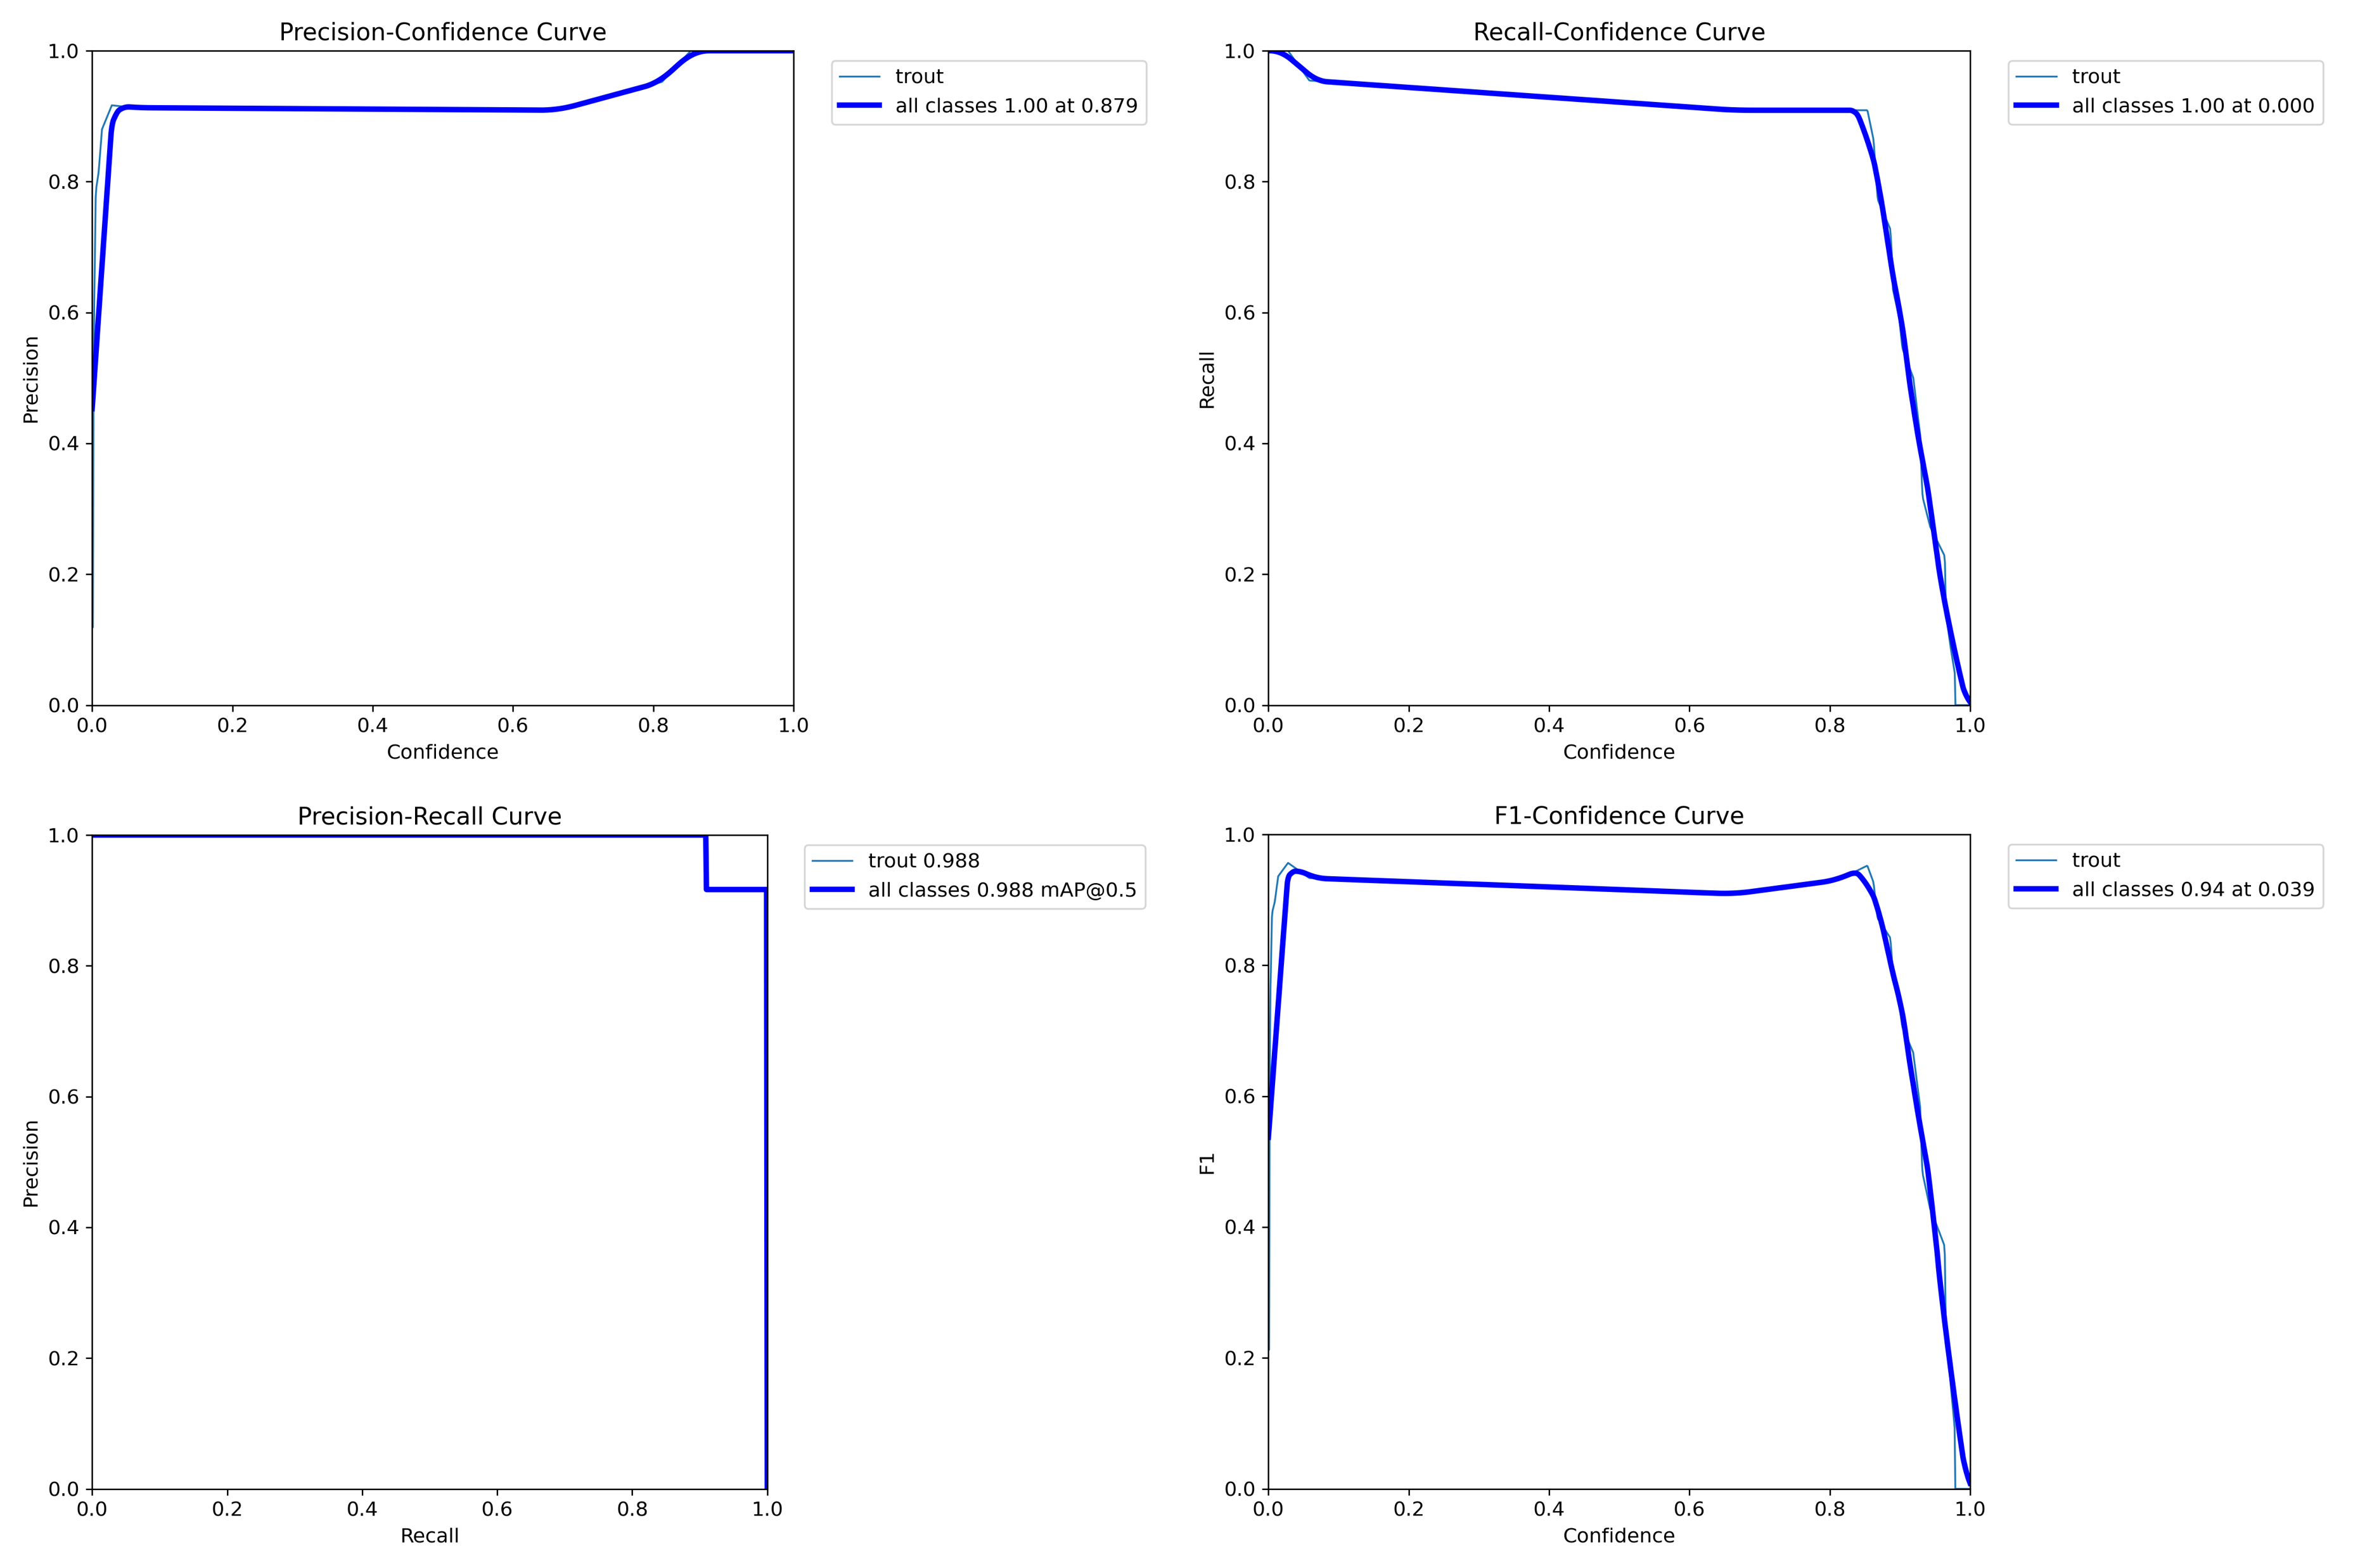
\includegraphics[width=0.9\textwidth]{images/13/b/4/graficas2.png}
        \caption{Gráficas de estadísticos finales del entrenamiento 4}
        \label{fig:Estadisticos4}
    \end{figure}
    \begin{figure}[H]
        \centering
        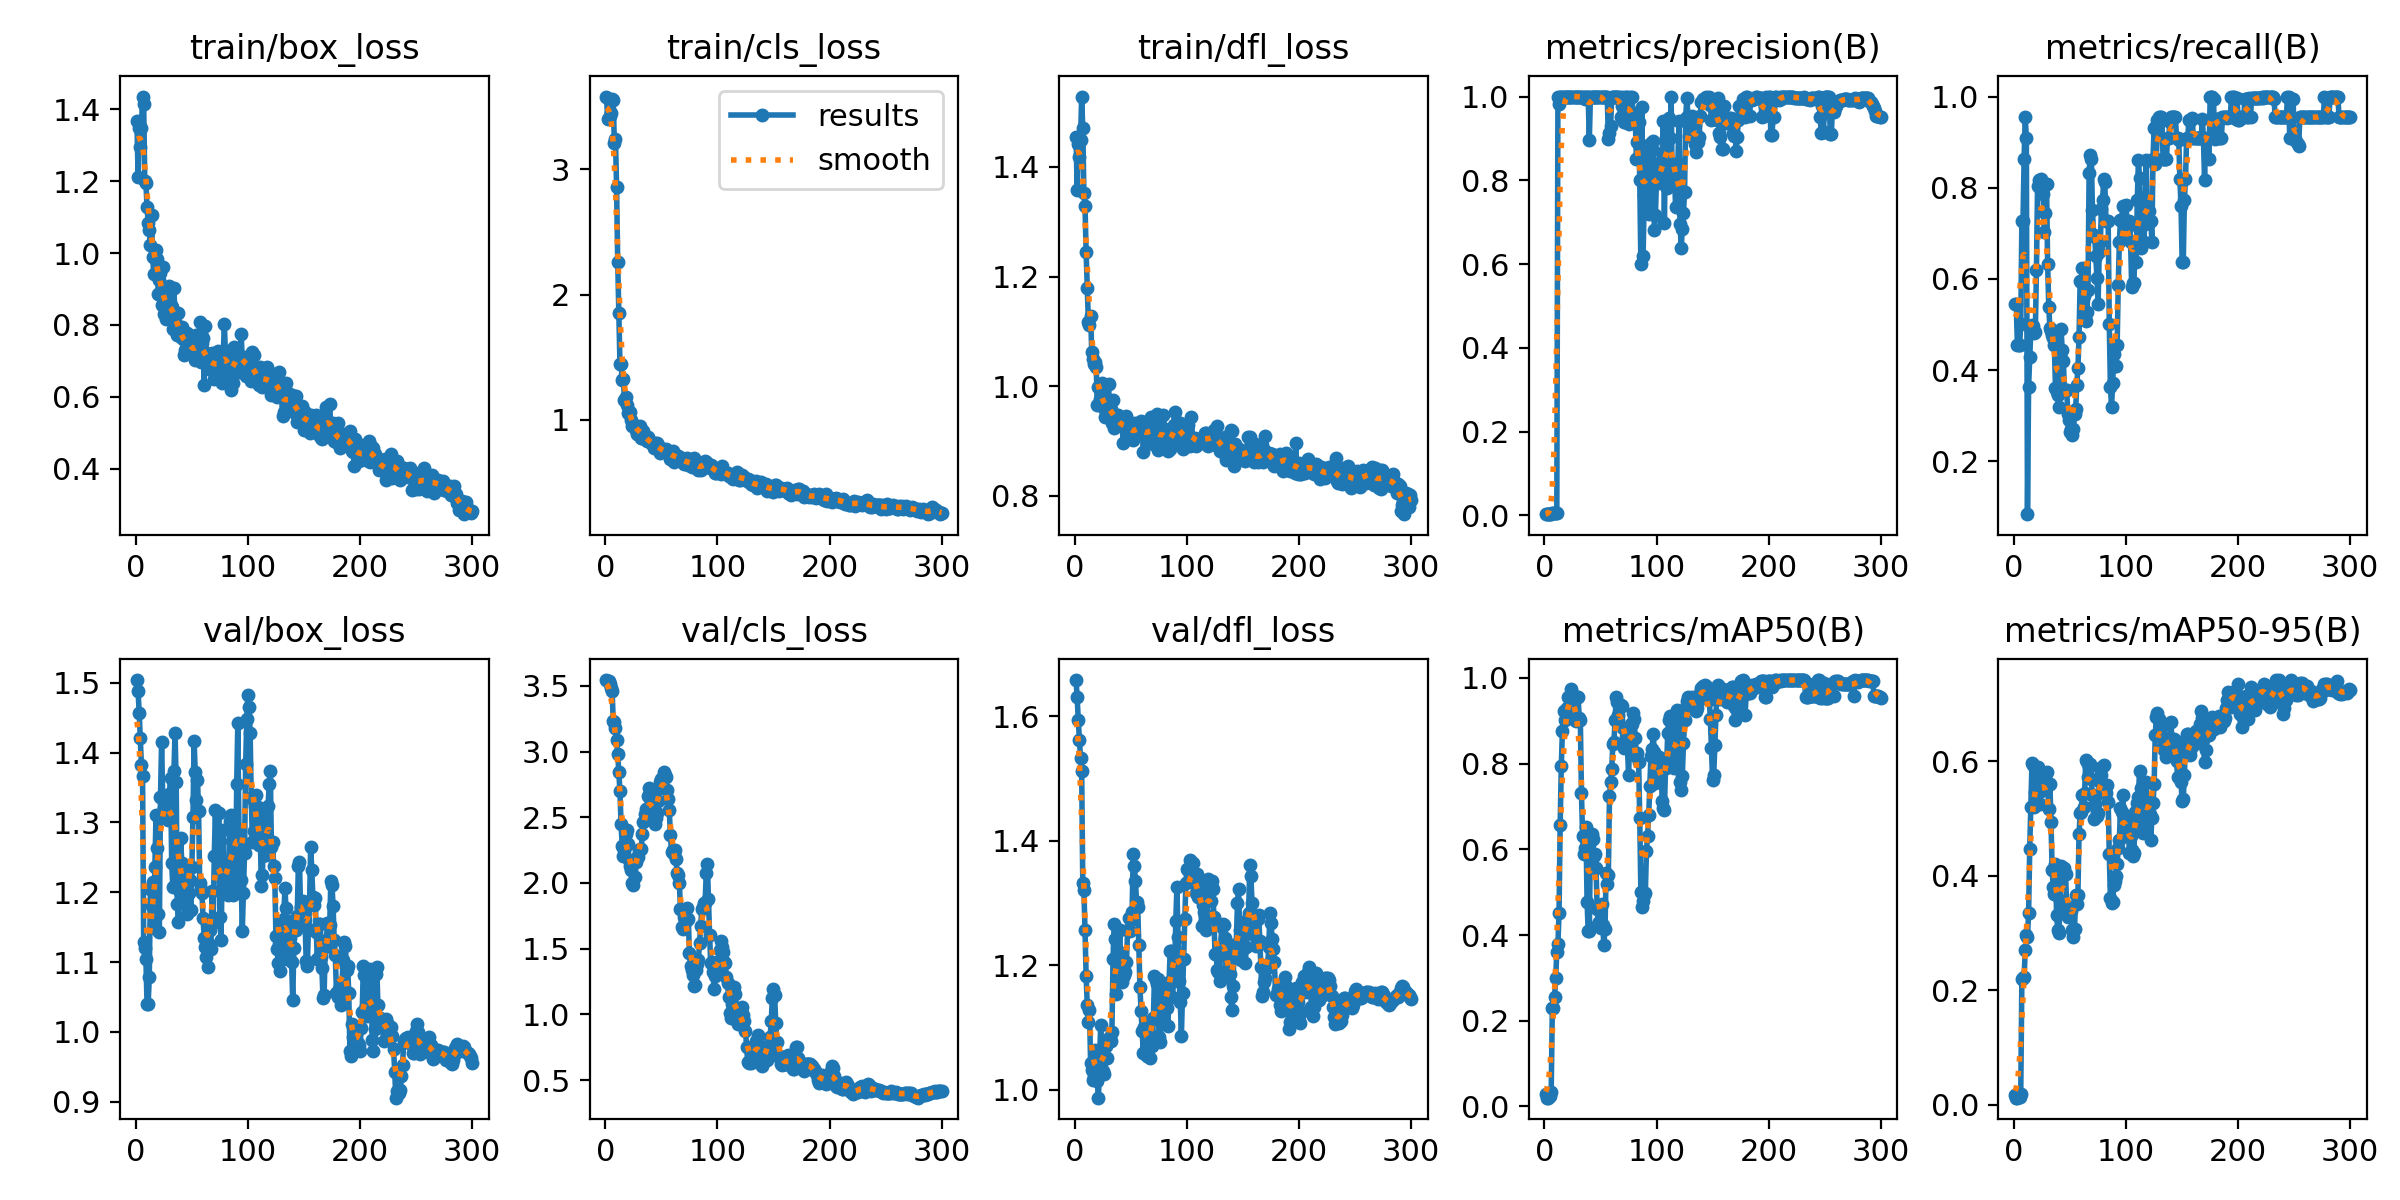
\includegraphics[width=0.9\textwidth]{images/13/b/4/results.png}
        \caption{Gráficas de evolución en épocas del entrenamiento 4}
        \label{fig:Resultados4}
    \end{figure}

\end{itemize}

\clearpage

\subsubsection*{Entrenamiento Final}
\label{train:final}
\begin{itemize}
    \item \textbf{Fecha}: 9 de junio de 2024.
    \item \textbf{Descripción del conjunto de datos}: 203 imágenes en total. Se añadieron fotogramas aleatorios de varios videos del experimento \textit{NetTest} para poder manejar un conjunto más grande.
    \item \textbf{Resultados del entrenamiento}: resultados muy positivos, sobre todo en la \autoref{fig:ResultadosFinal} en la confianza con la que se realizan las clasificaciones y la curva F1, que aún siendo mejorable, solo tiene problemas 
    con falsos positivos en valores de confianza muy altos. Aparte de esto, como se puede apreciar en la \autoref{fig:EstadisticosFinal}, el error de aproximación a la \texttt{Bounding Box} predicha se ha 
    conseguido reducir mucho tanto en entrenamiento como en el conjunto de validación, que es principalmente lo que se necesitaba del modelo \texttt{YOLO} para este trabajo.
    
    \begin{figure}[H]
        \centering
        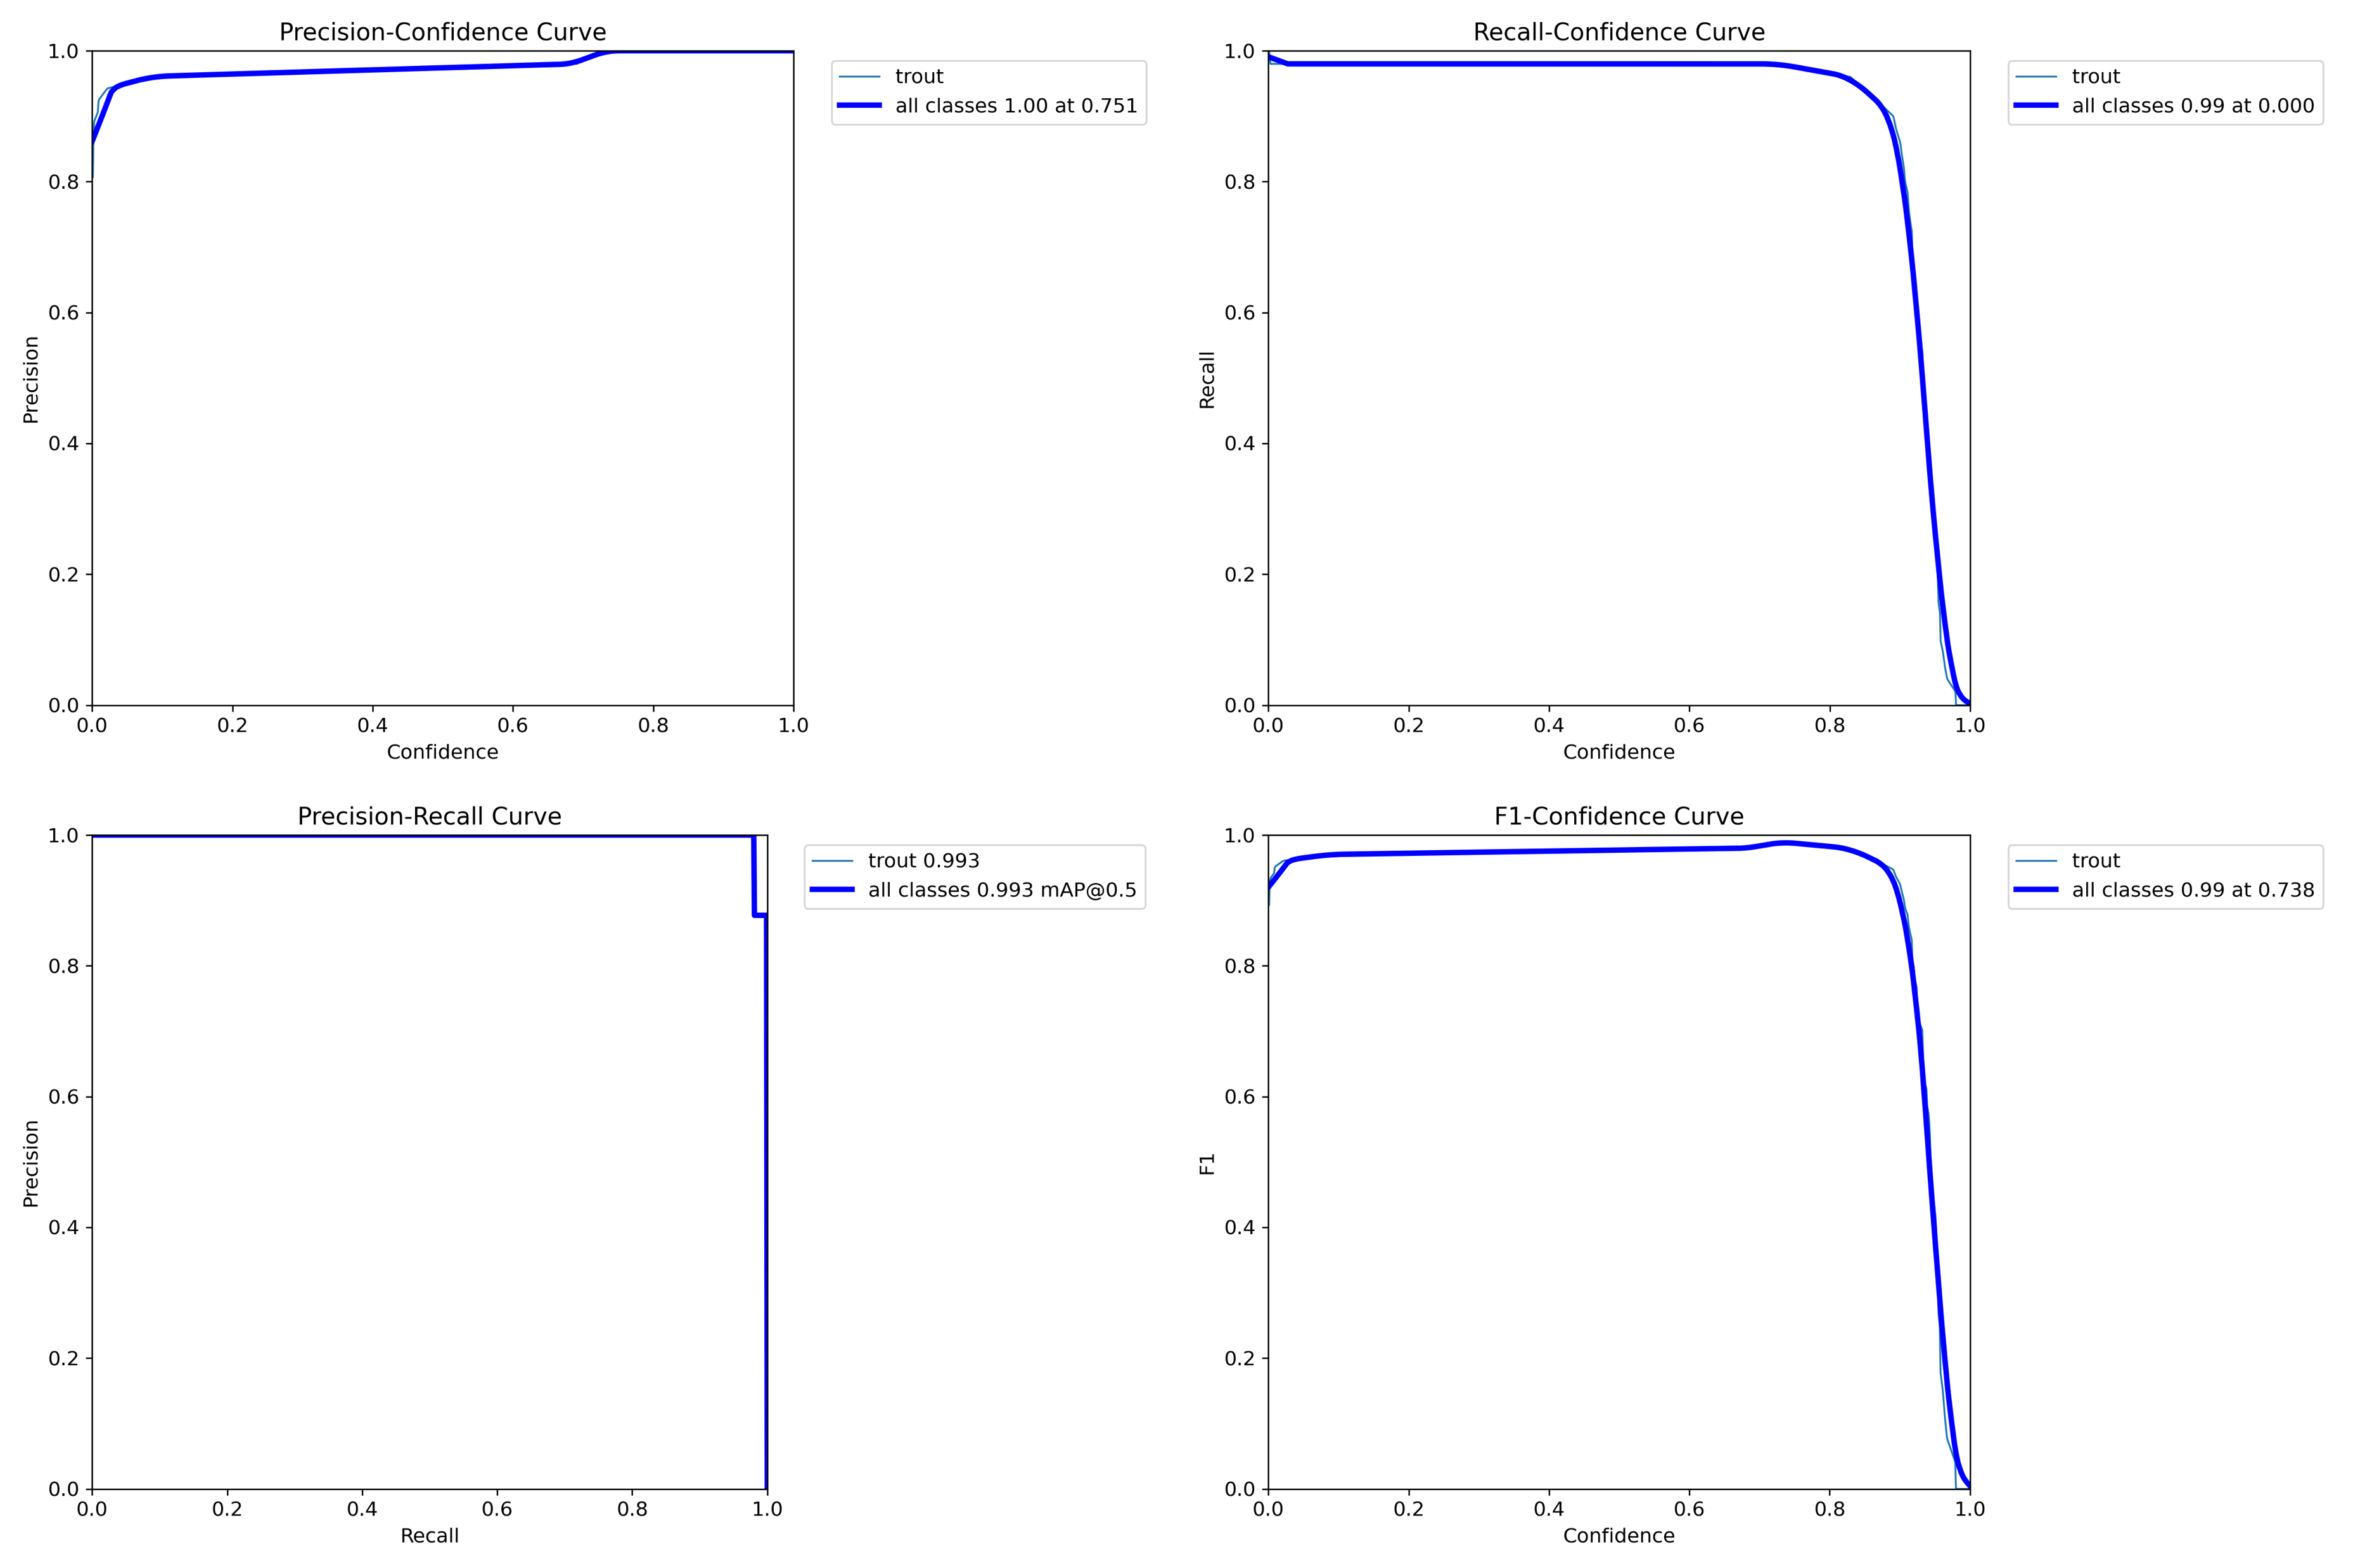
\includegraphics[width=0.9\textwidth]{images/13/b/final/graficas2.png}
        \caption{Gráficas de estadísticos del último entrenamiento}
        \label{fig:EstadisticosFinal}
    \end{figure}
    \begin{figure}[H]
        \centering
        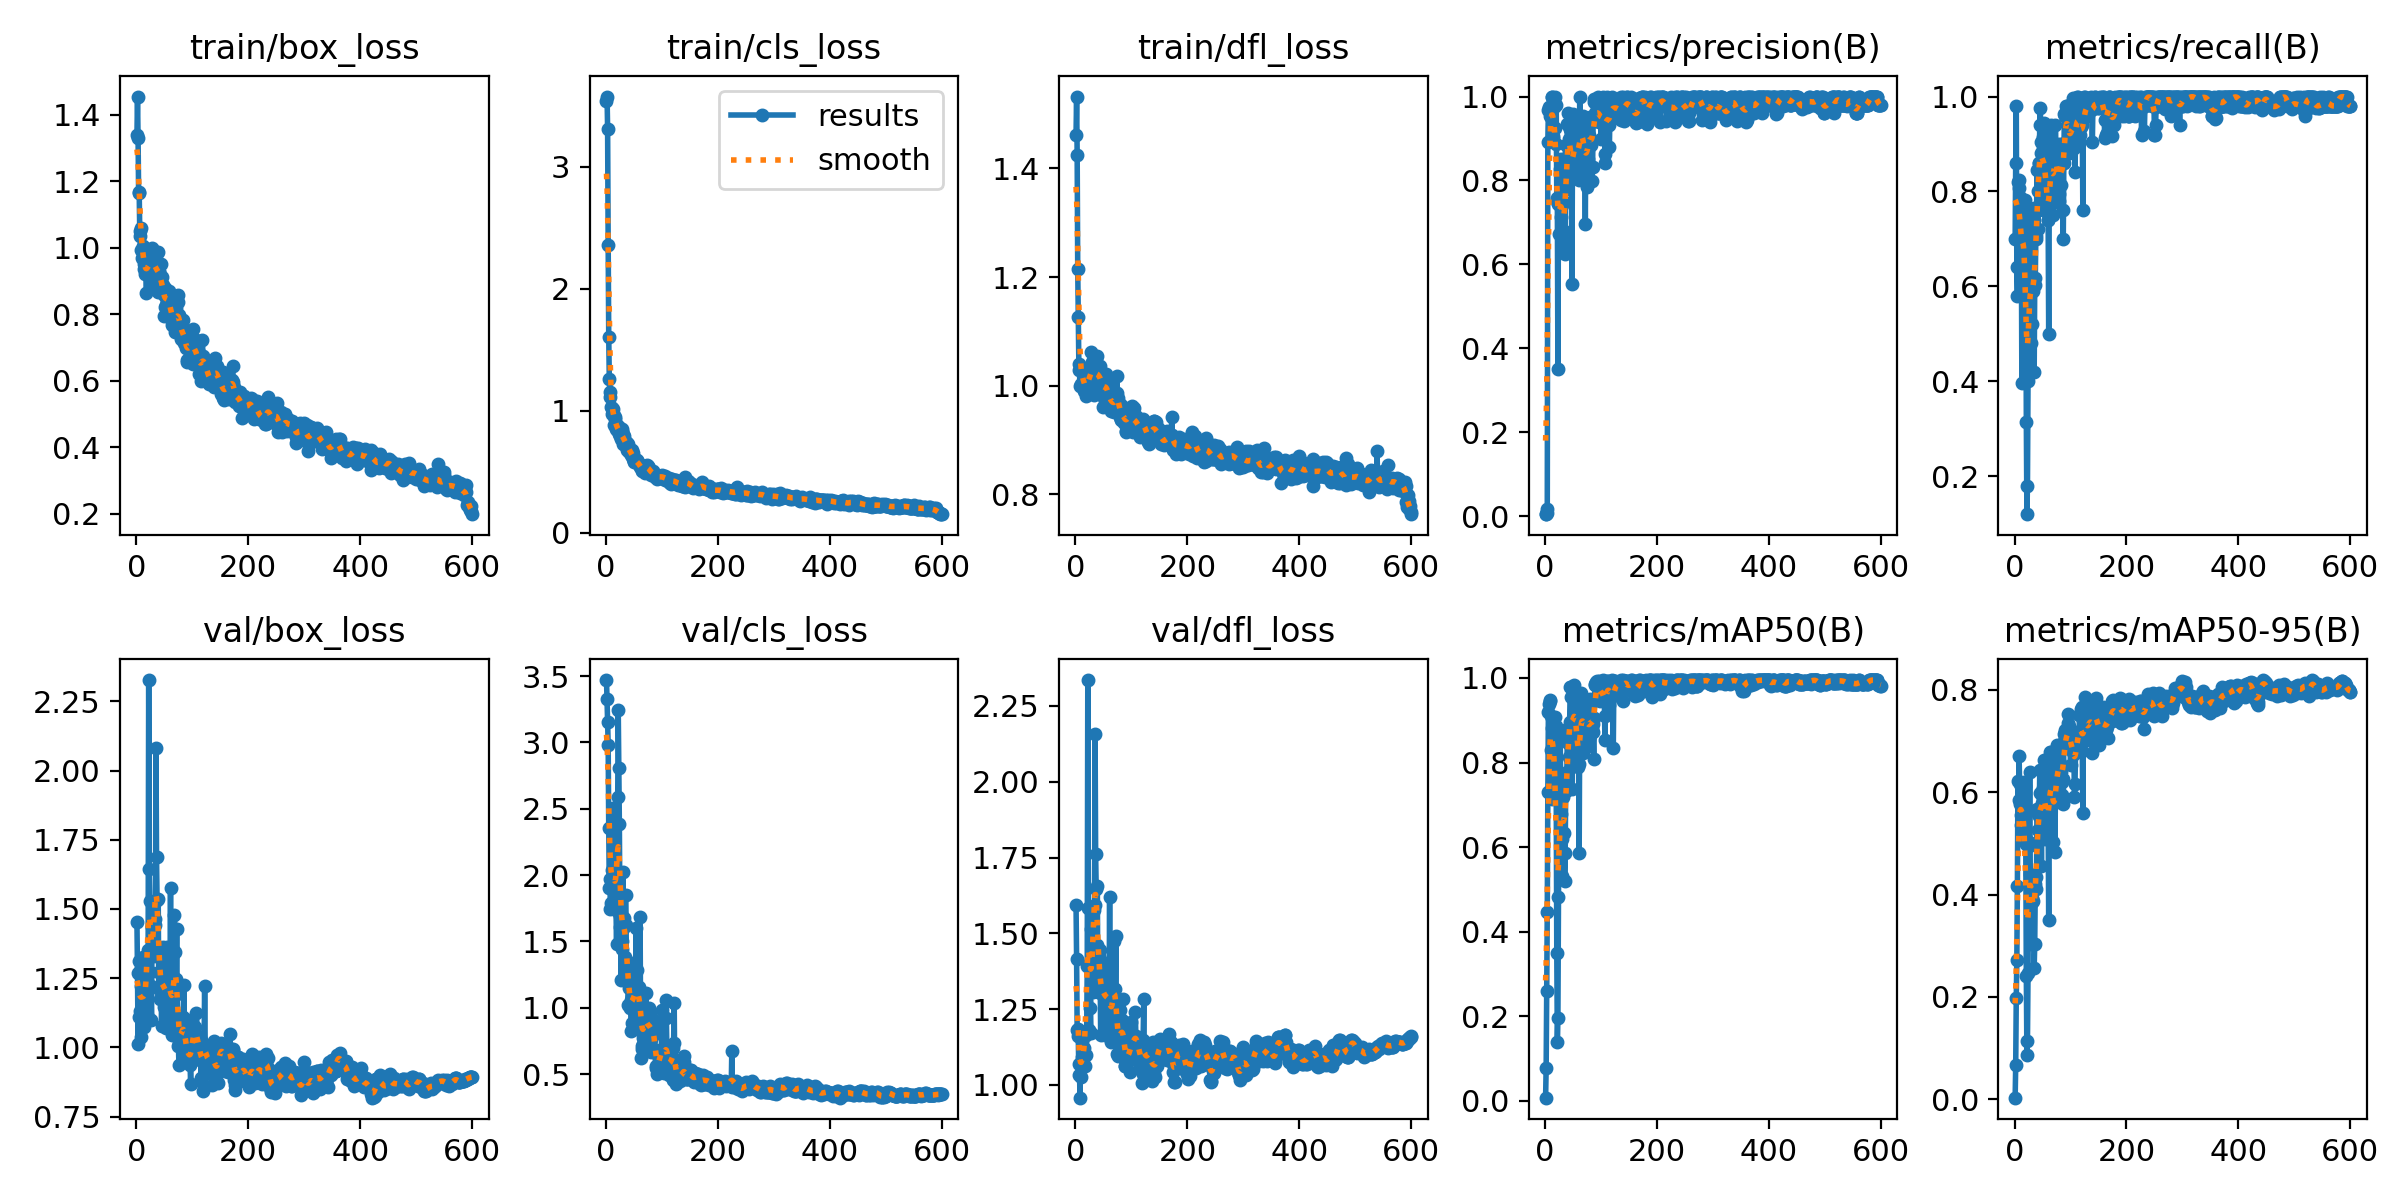
\includegraphics[width=0.9\textwidth]{images/13/b/final/results.png}
        \caption{Gráficas de evolución en épocas del último entrenamiento}
        \label{fig:ResultadosFinal}
    \end{figure}
\end{itemize}

\clearpage

\subsubsection*{Entrenamiento OBB}
\label{OBB:1}
\begin{itemize}
    \item \textbf{Fecha}: 9 de mayo de 2024.
    \item \textbf{Descripción del conjunto de datos}: conjunto común al \hyperref[train:4]{entrenamiento 4}, 84 imágenes tanto de videos nuevos como de videos antiguos.
    \item \textbf{Resultados del entrenamiento}: se observan los problemas que conllevan trabajar con \texttt{Bounding Boxes} orientadas, se pierde mucho tanto en métricas como en rendimiento general. 
    El punto positivo de este sistema es acotar lo máximo posible la \texttt{Bounding Box} al elemento, pero principalmente se observa una dificultad añadida y necesidad de mucho más entrenamiento y 
    ajuste de hiperparámetros para conseguir sobre todo mejorar el \acrshort{map}50-95.

    \begin{figure}[H]
        \centering
        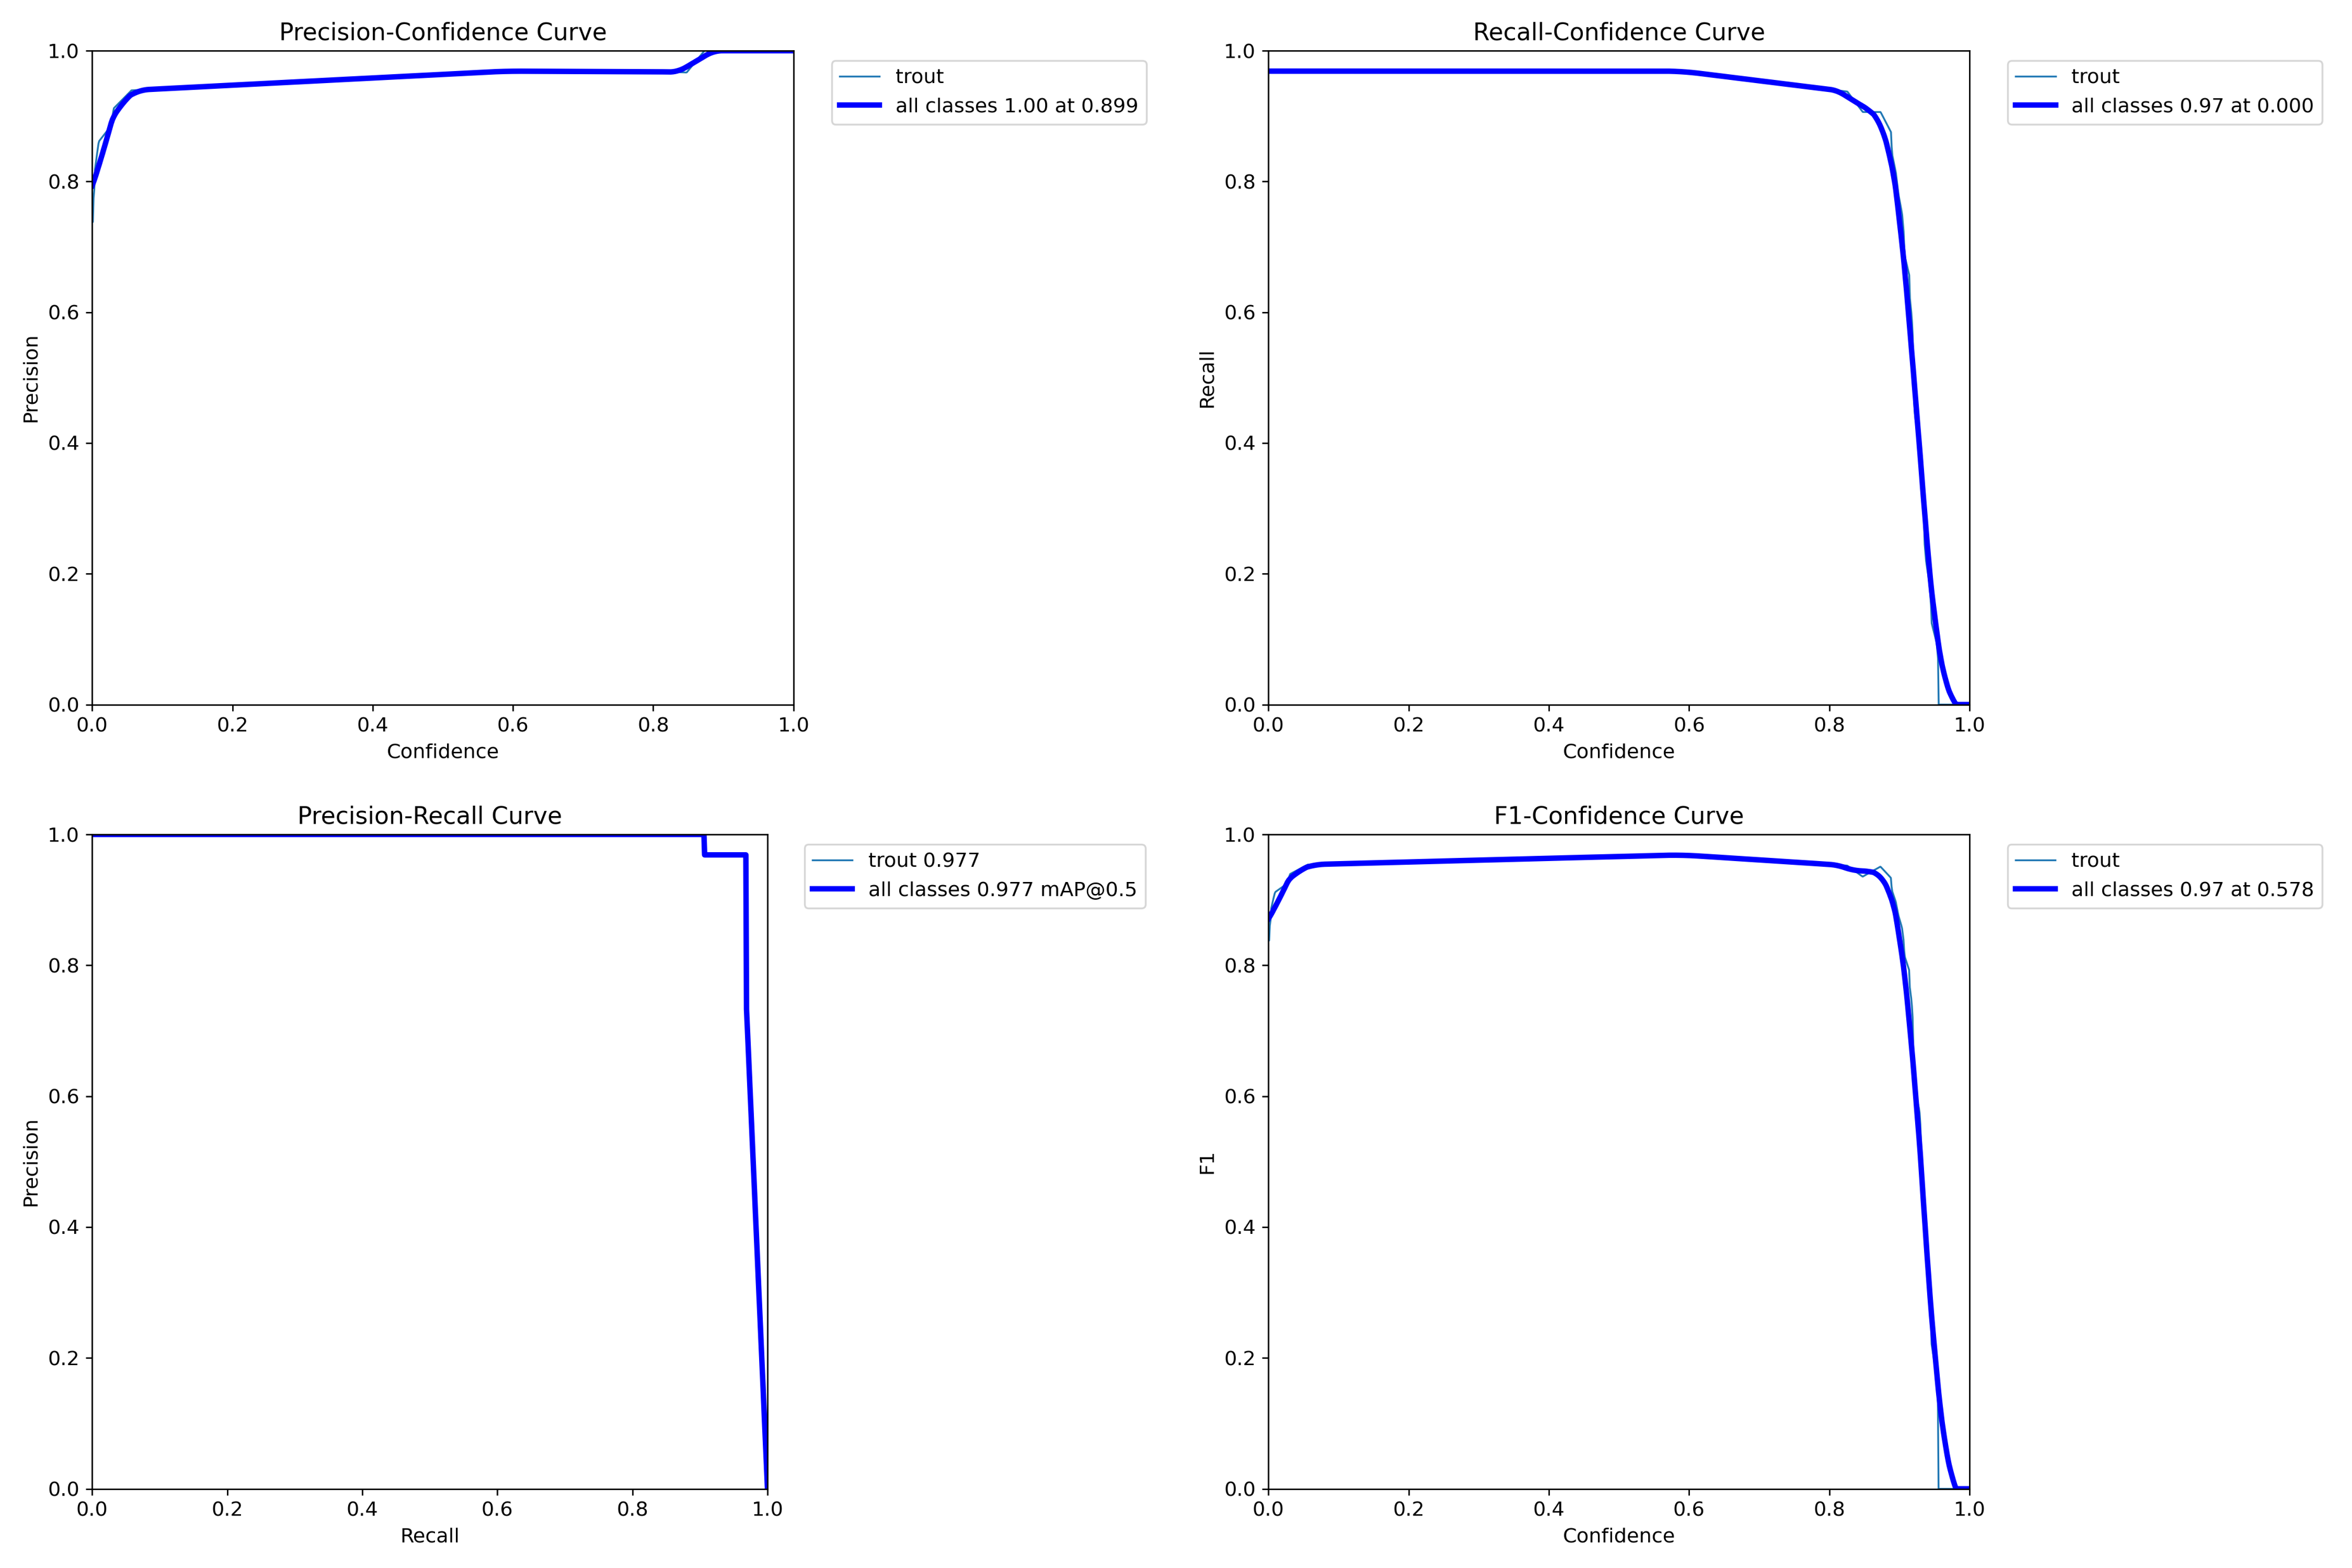
\includegraphics[width=0.9\textwidth]{images/13/b/obb/graficas2.png}
        \caption{Gráficas de estadísticos finales del entrenamiento \texttt{OBB}}
        \label{fig:EstadisticosOBB}
    \end{figure}
    \begin{figure}[H]
        \centering
        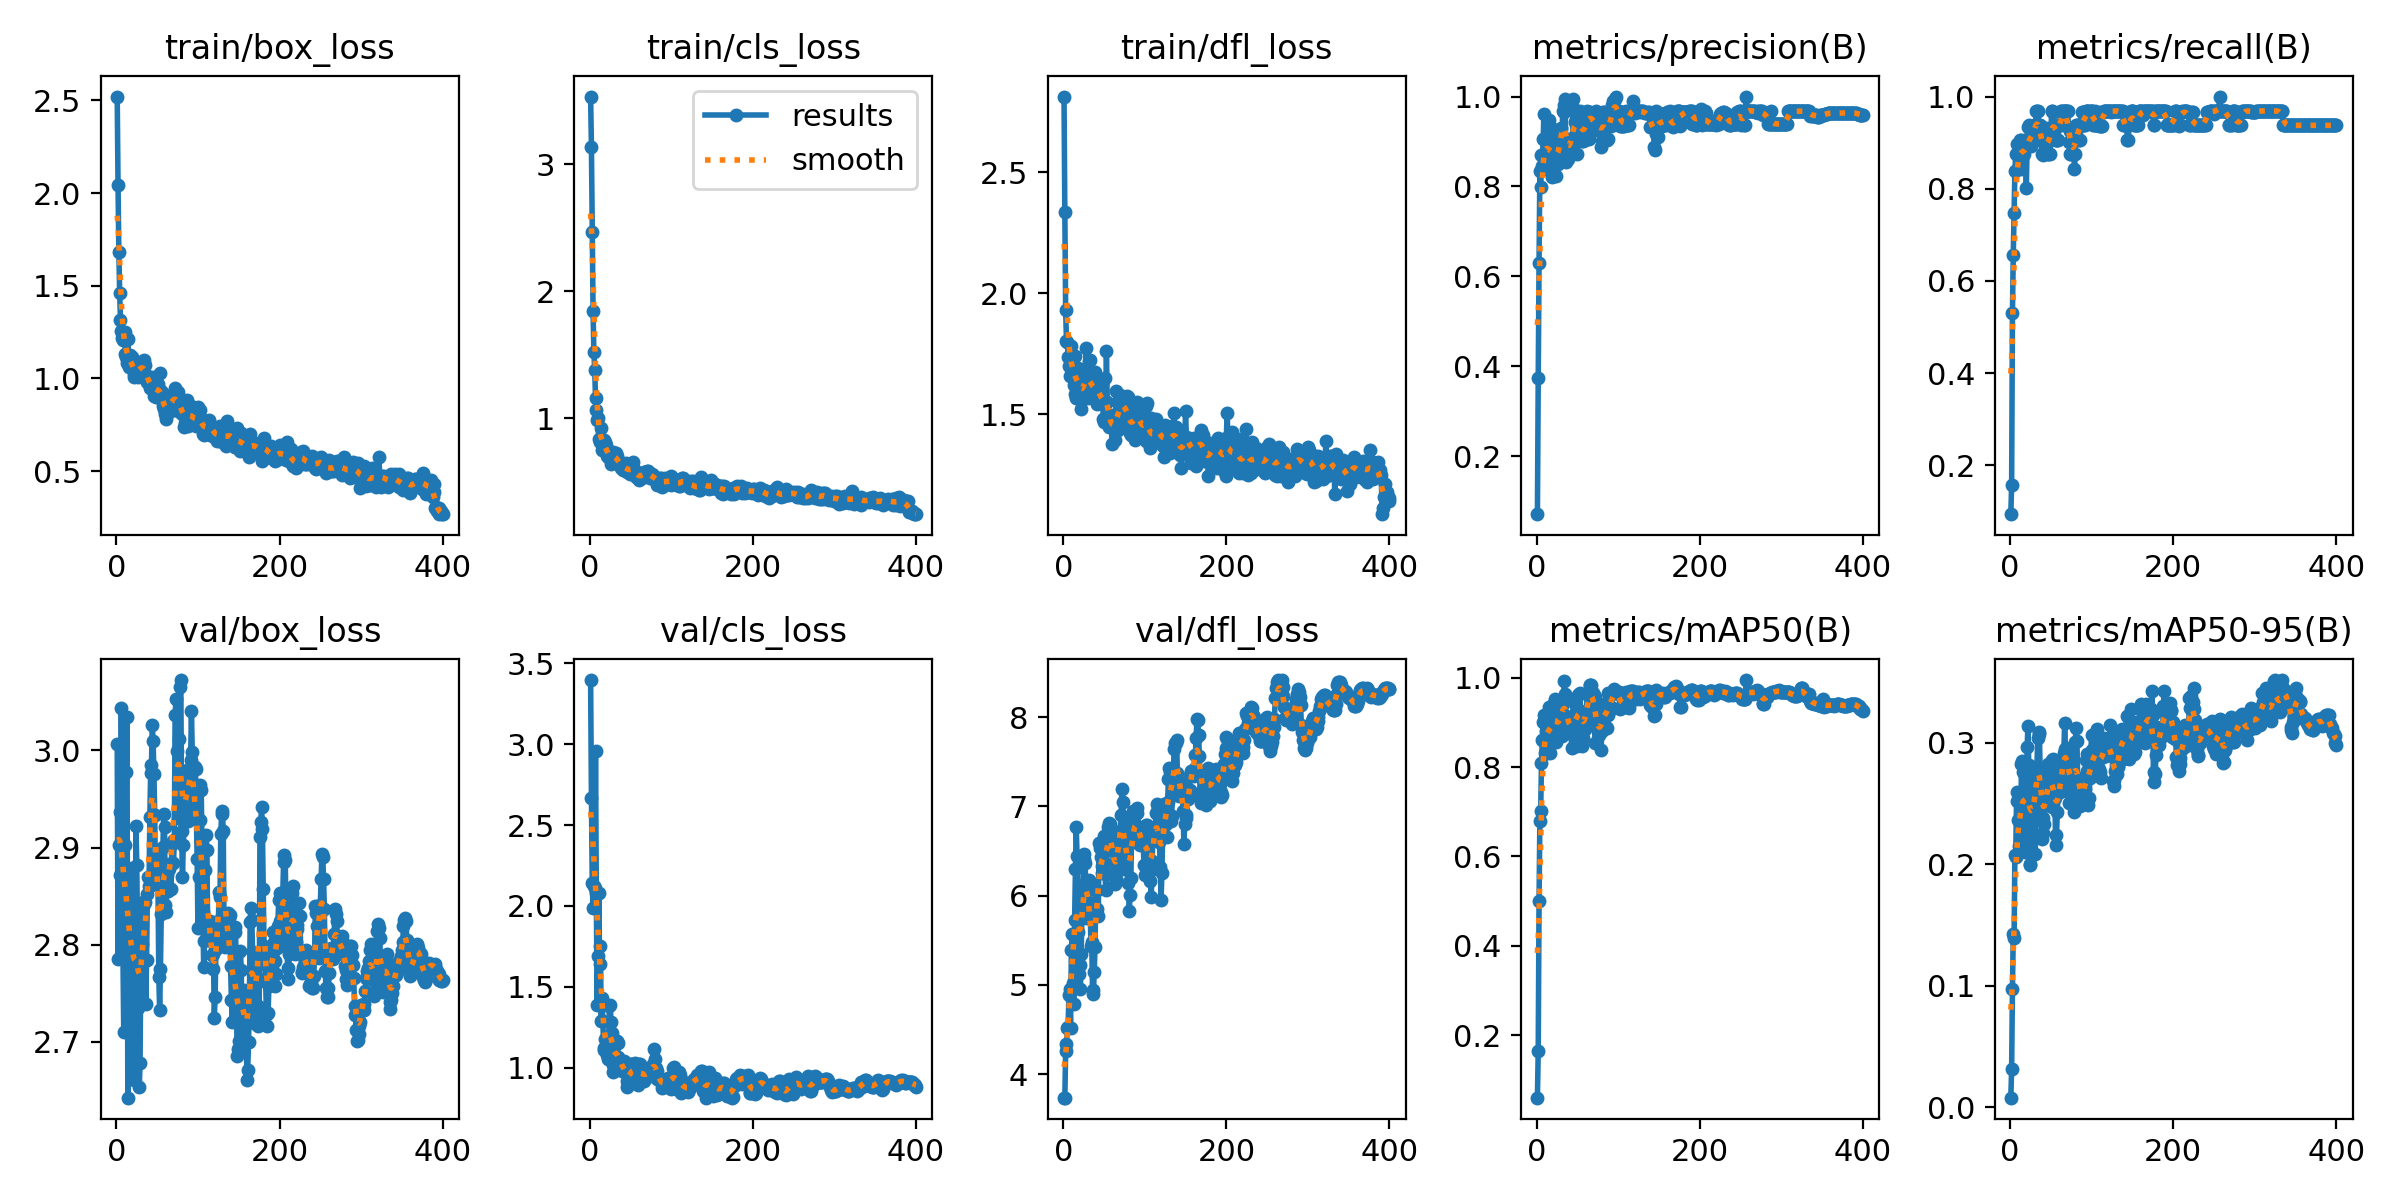
\includegraphics[width=0.9\textwidth]{images/13/b/obb/results.png}
        \caption{Gráficas de evolución en épocas del entrenamiento \texttt{OBB}}
        \label{fig:ResultadosOBB}
    \end{figure}

\end{itemize}
\clearpage
\subsection*{ANEXO C: Diagramas de diseño}
\subsubsection*{Esquema de flujo y ventanas de \acrshort{gui}}
\label{esquema:FlujoVentanas}
\begin{figure}[H]
    \centering
    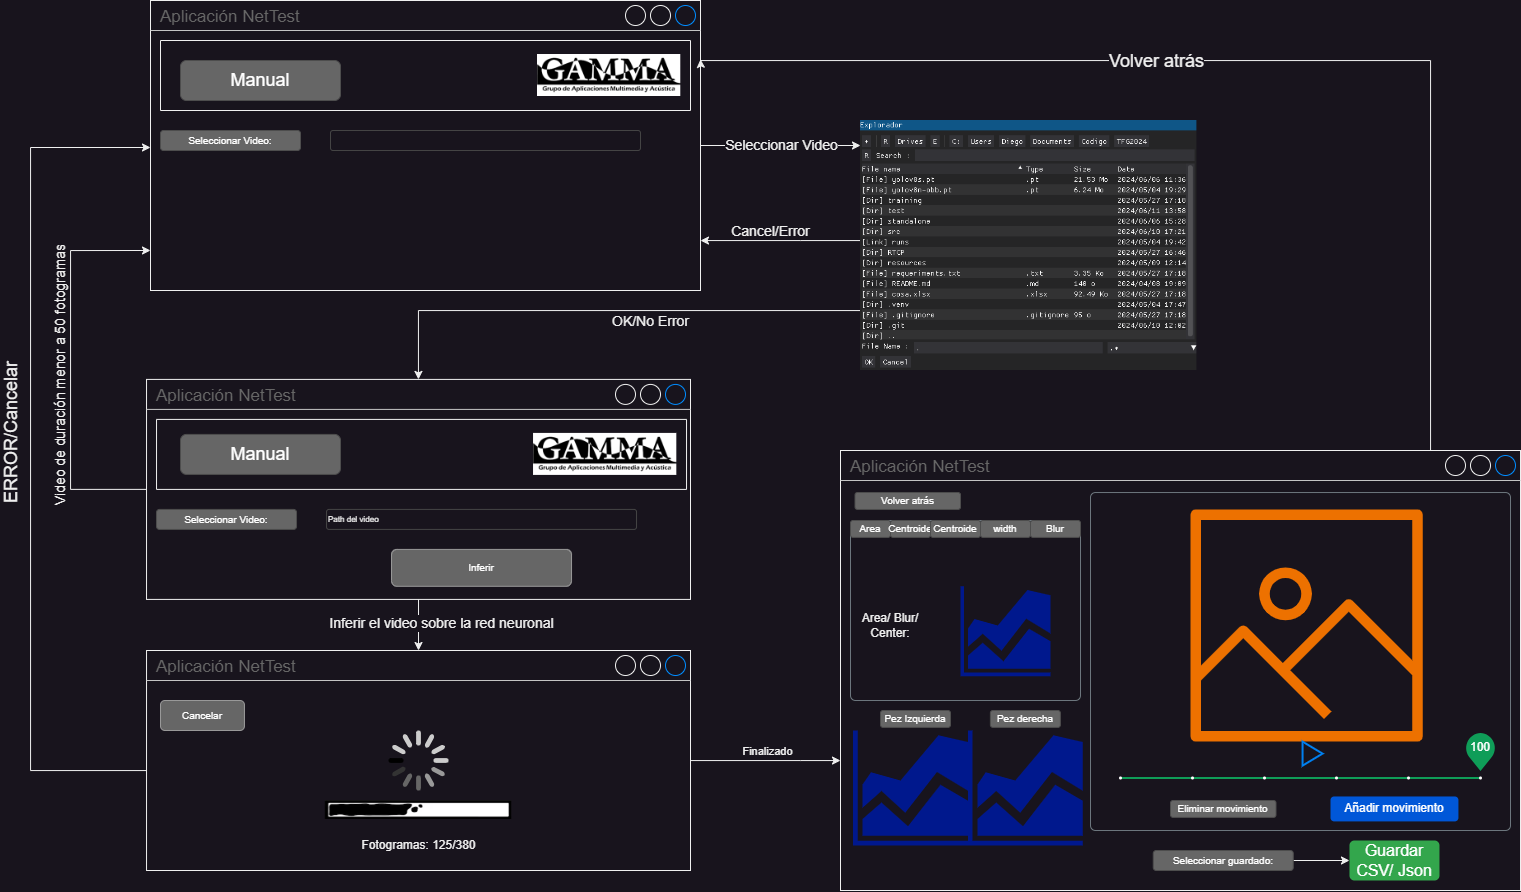
\includegraphics[angle=90,origin=c,width=0.85\textwidth]{images/13/c/Interfaz.png}
    \caption{Esquema de flujo y ventanas de la aplicación}
    \label{fig:FlujoVentanas}
\end{figure}
\clearpage
\subsubsection*{Diagrama de clases de la aplicación}
\label{esquema:DiagramaClases}
\begin{figure}[H]
    \centering
    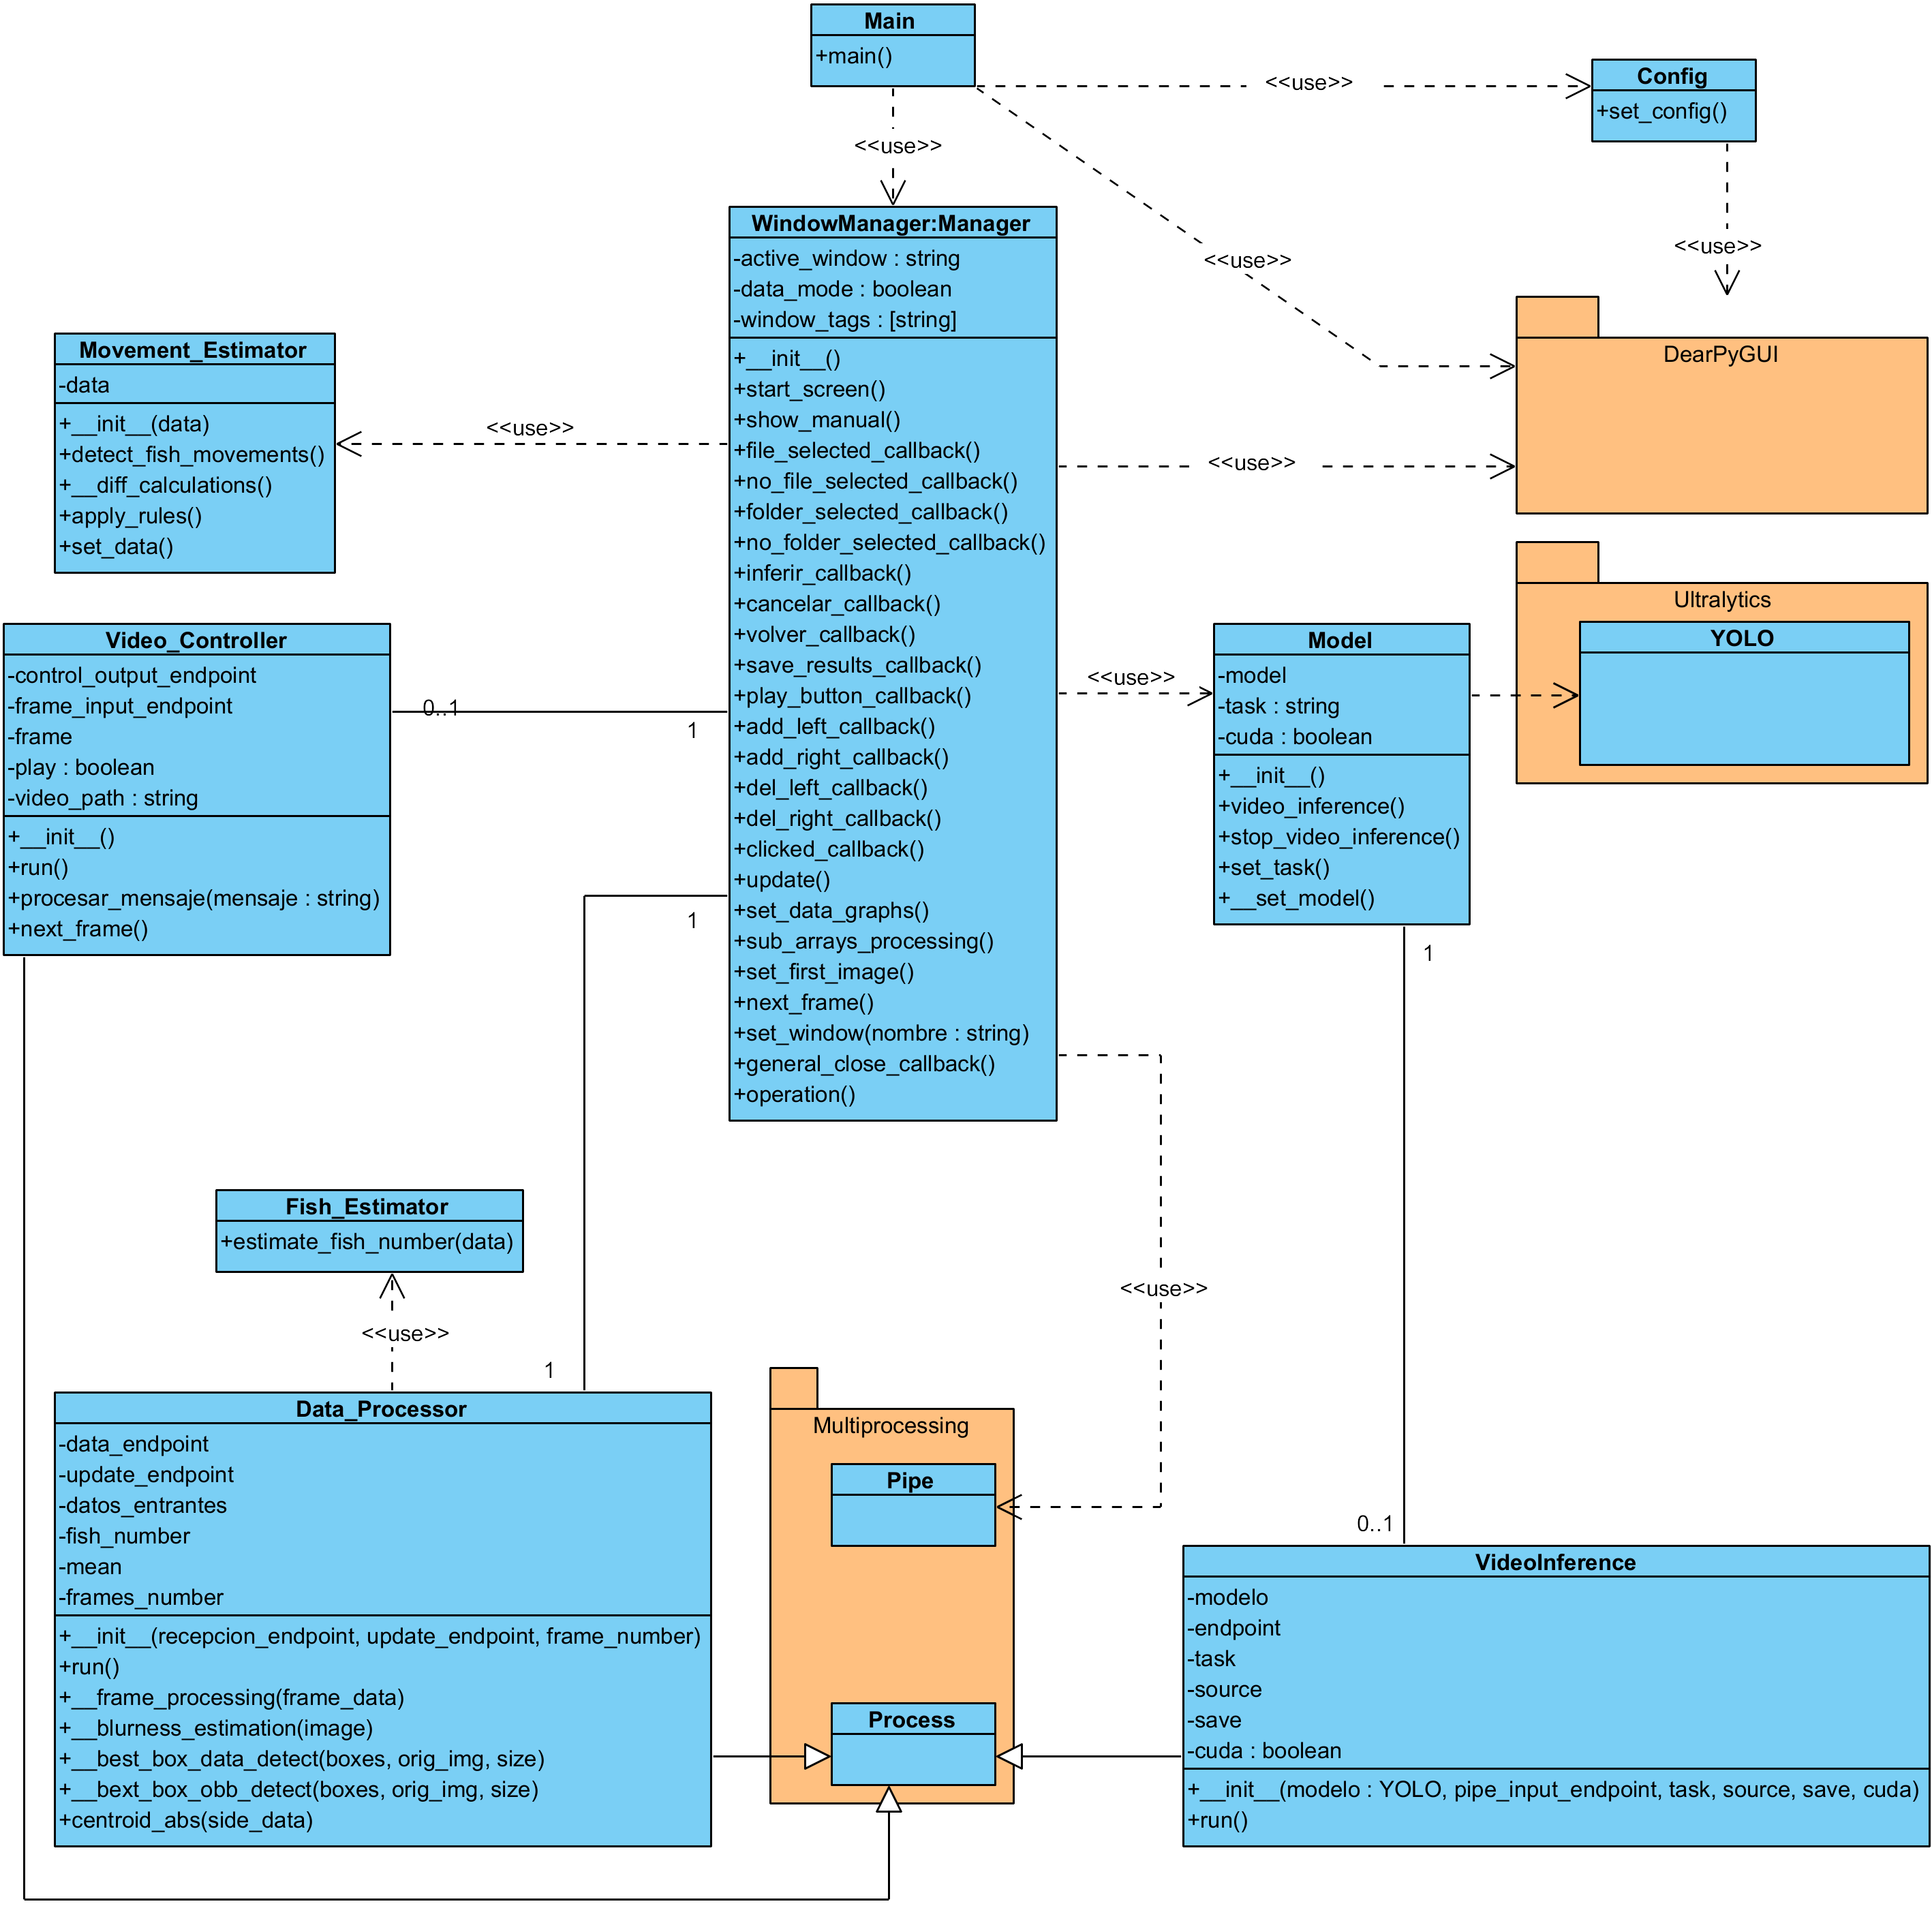
\includegraphics[width=\textwidth]{images/13/c/ClasesTFG.png}
    \caption{Diagrama de clases de la aplicación}
    \label{fig:DiagramaClases}
\end{figure}
\subsubsection*{Diagramas de secuencia}
\label{esquema:SecuenciaInferir}
\begin{figure}[H]
    \centering
    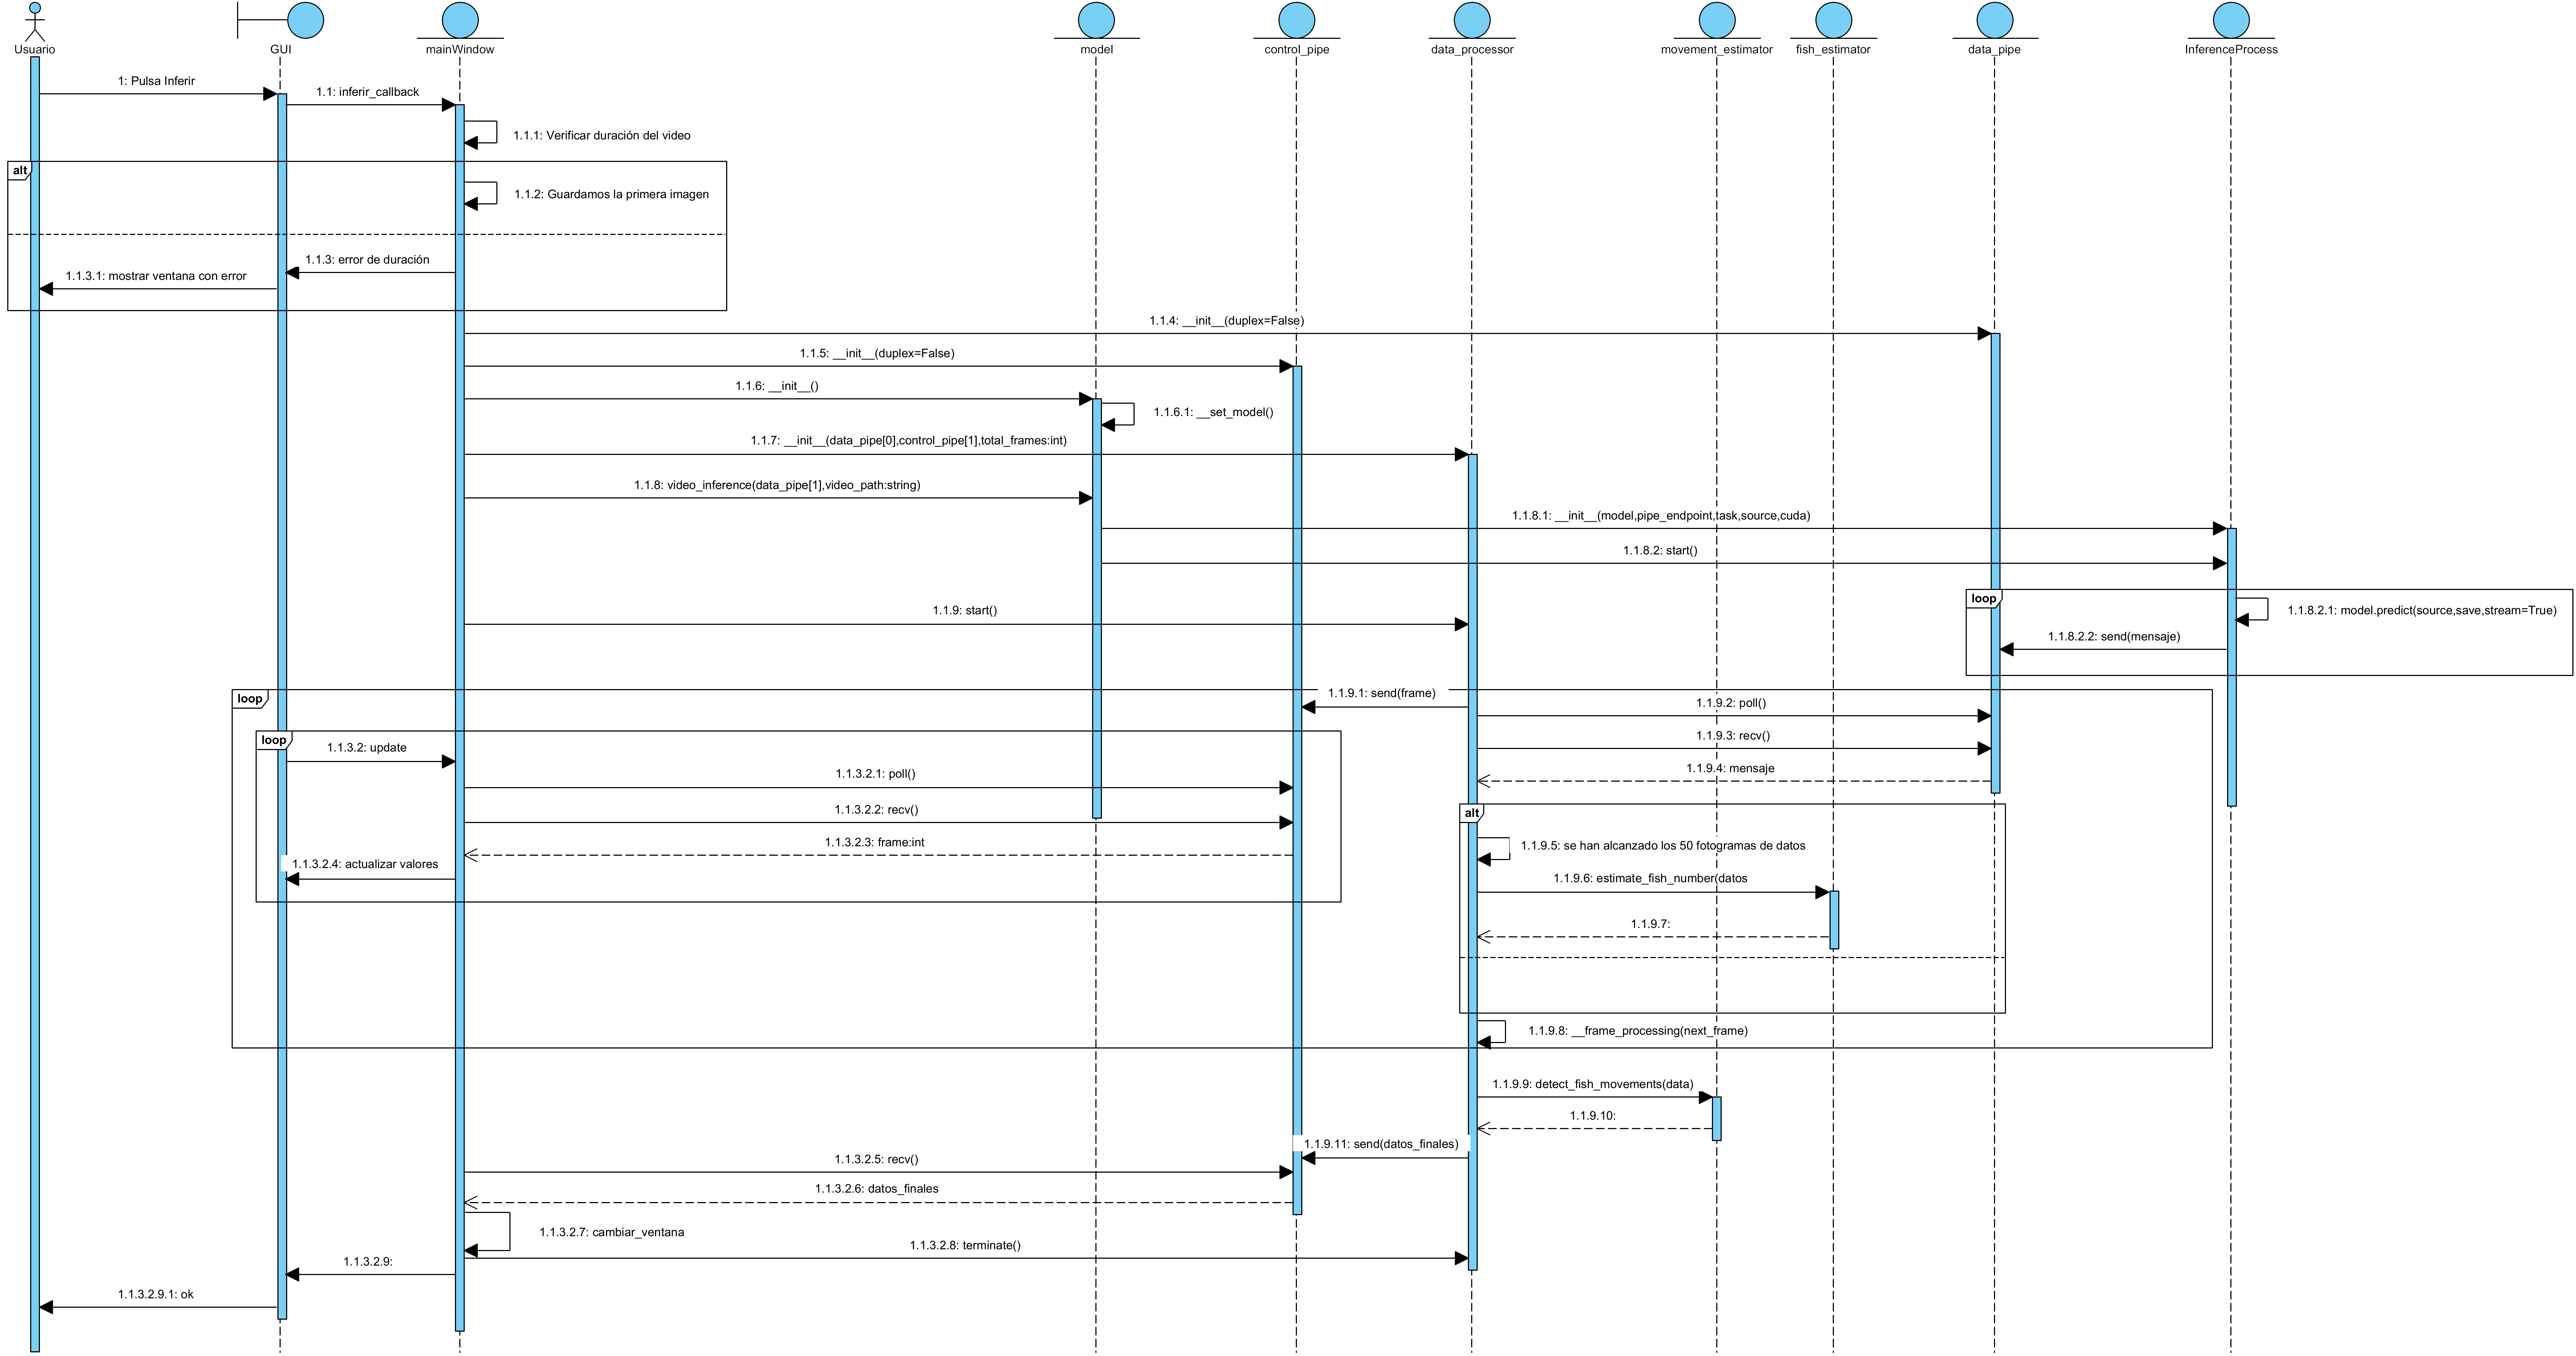
\includegraphics[angle=90,origin=c,width=0.80\textwidth]{images/13/c/Inferir.png}
    \caption{Diagrama de secuencia en el caso de uso de pulsar el botón de inferir}
\end{figure}
\clearpage
\label{esquema:SecuenciaResto}
\begin{figure}[H]
    \centering
    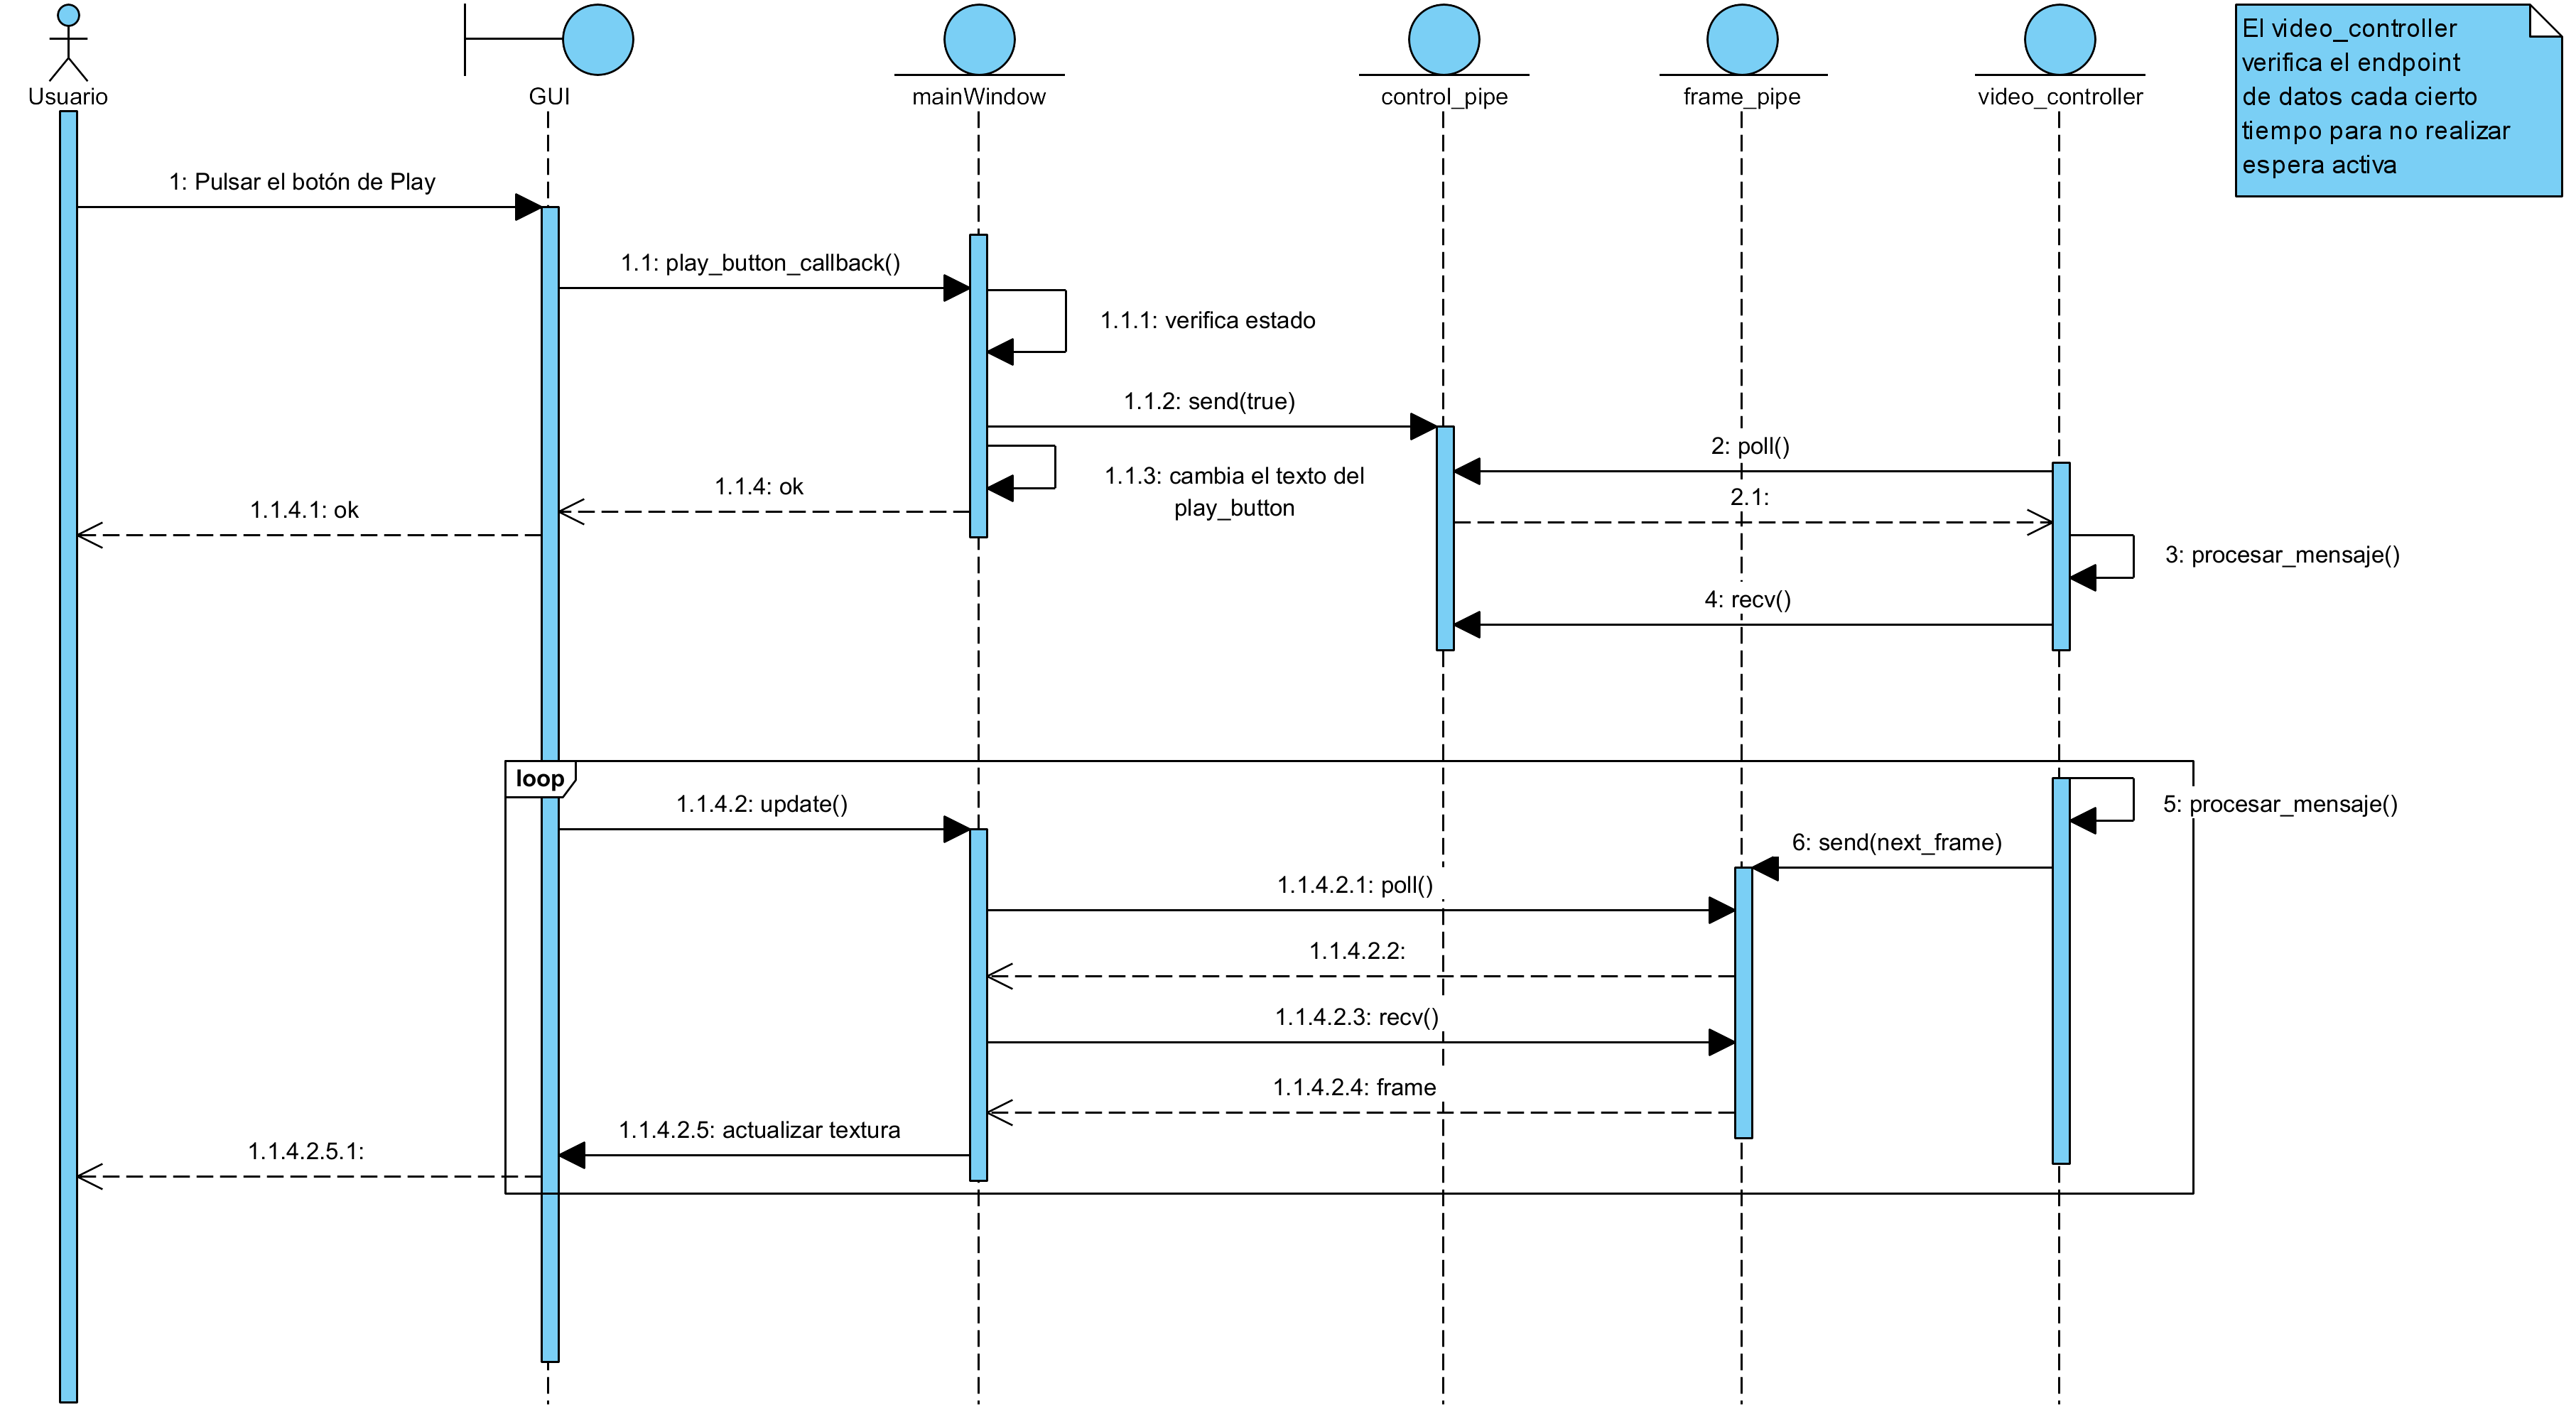
\includegraphics[width=\textwidth]{images/13/c/Play.png}
    \caption{Diagrama de secuencia en el caso de uso de pulsar el botón de reproducción}
\end{figure}
\begin{figure}[H]
    \centering
    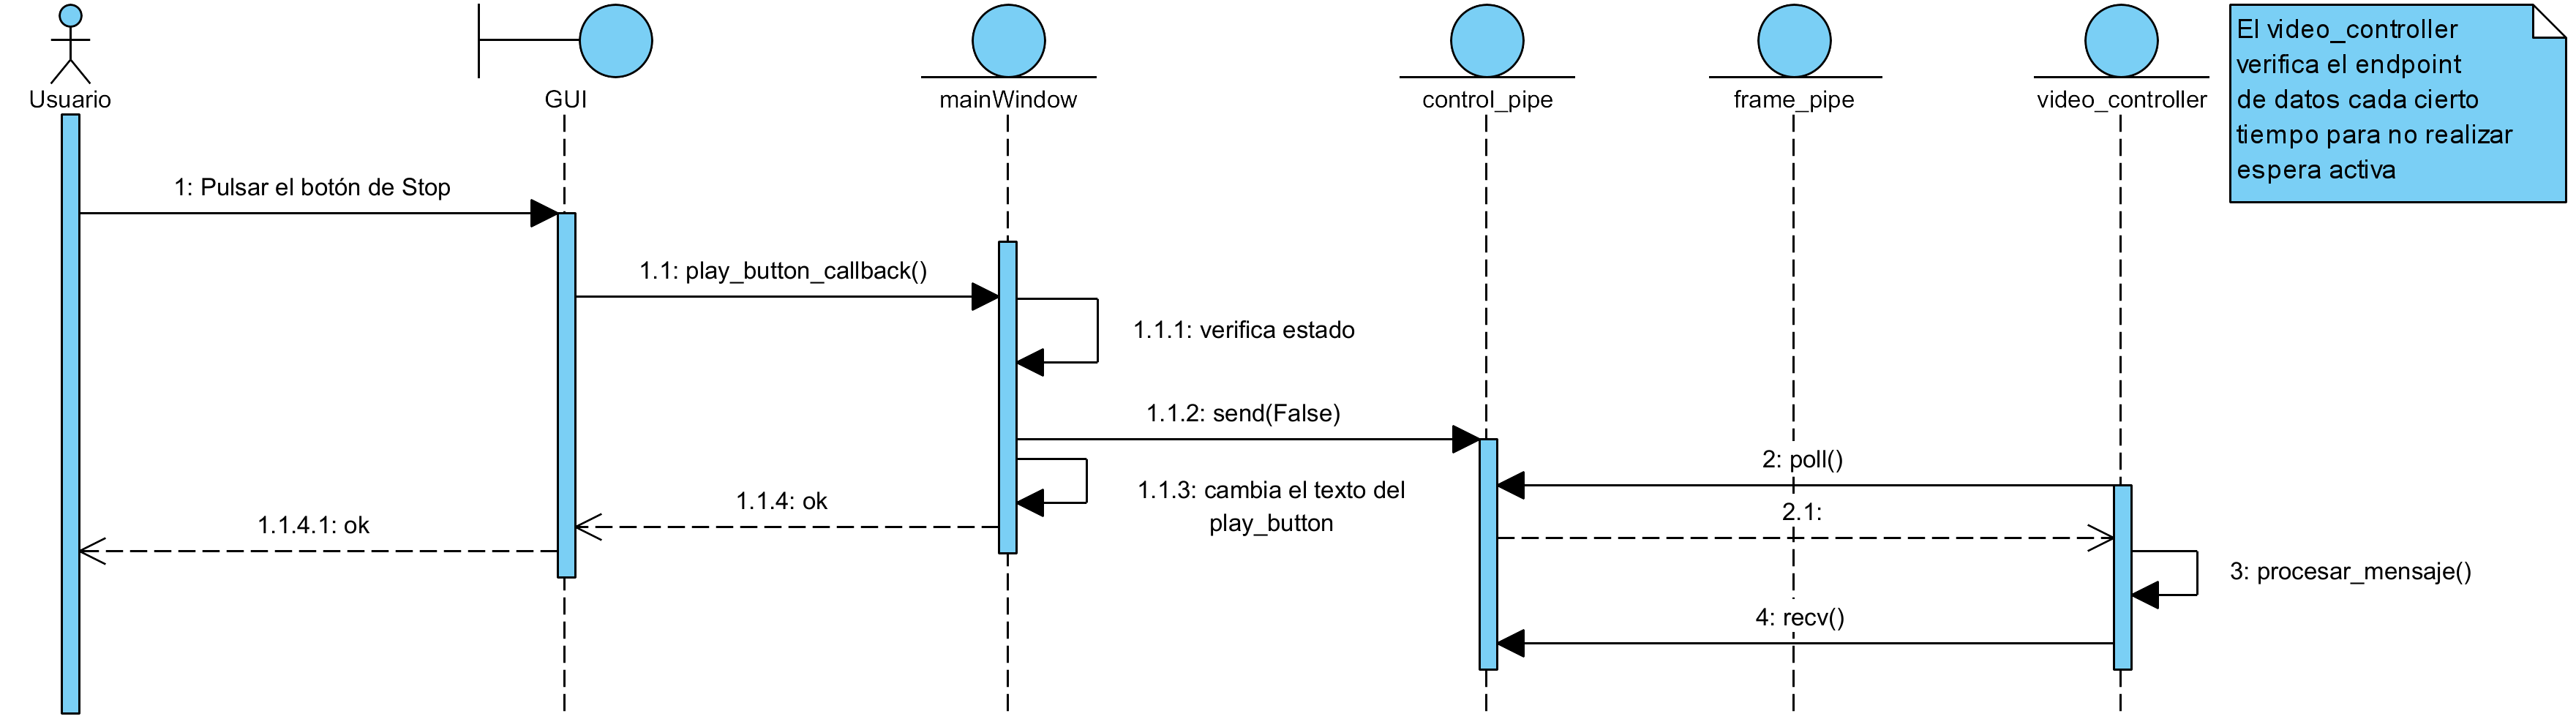
\includegraphics[width=\textwidth]{images/13/c/Stop.png}
    \caption{Diagrama de secuencia en el caso de uso de pulsar el botón de pausa}
\end{figure}
\begin{figure}[H]
    \centering
    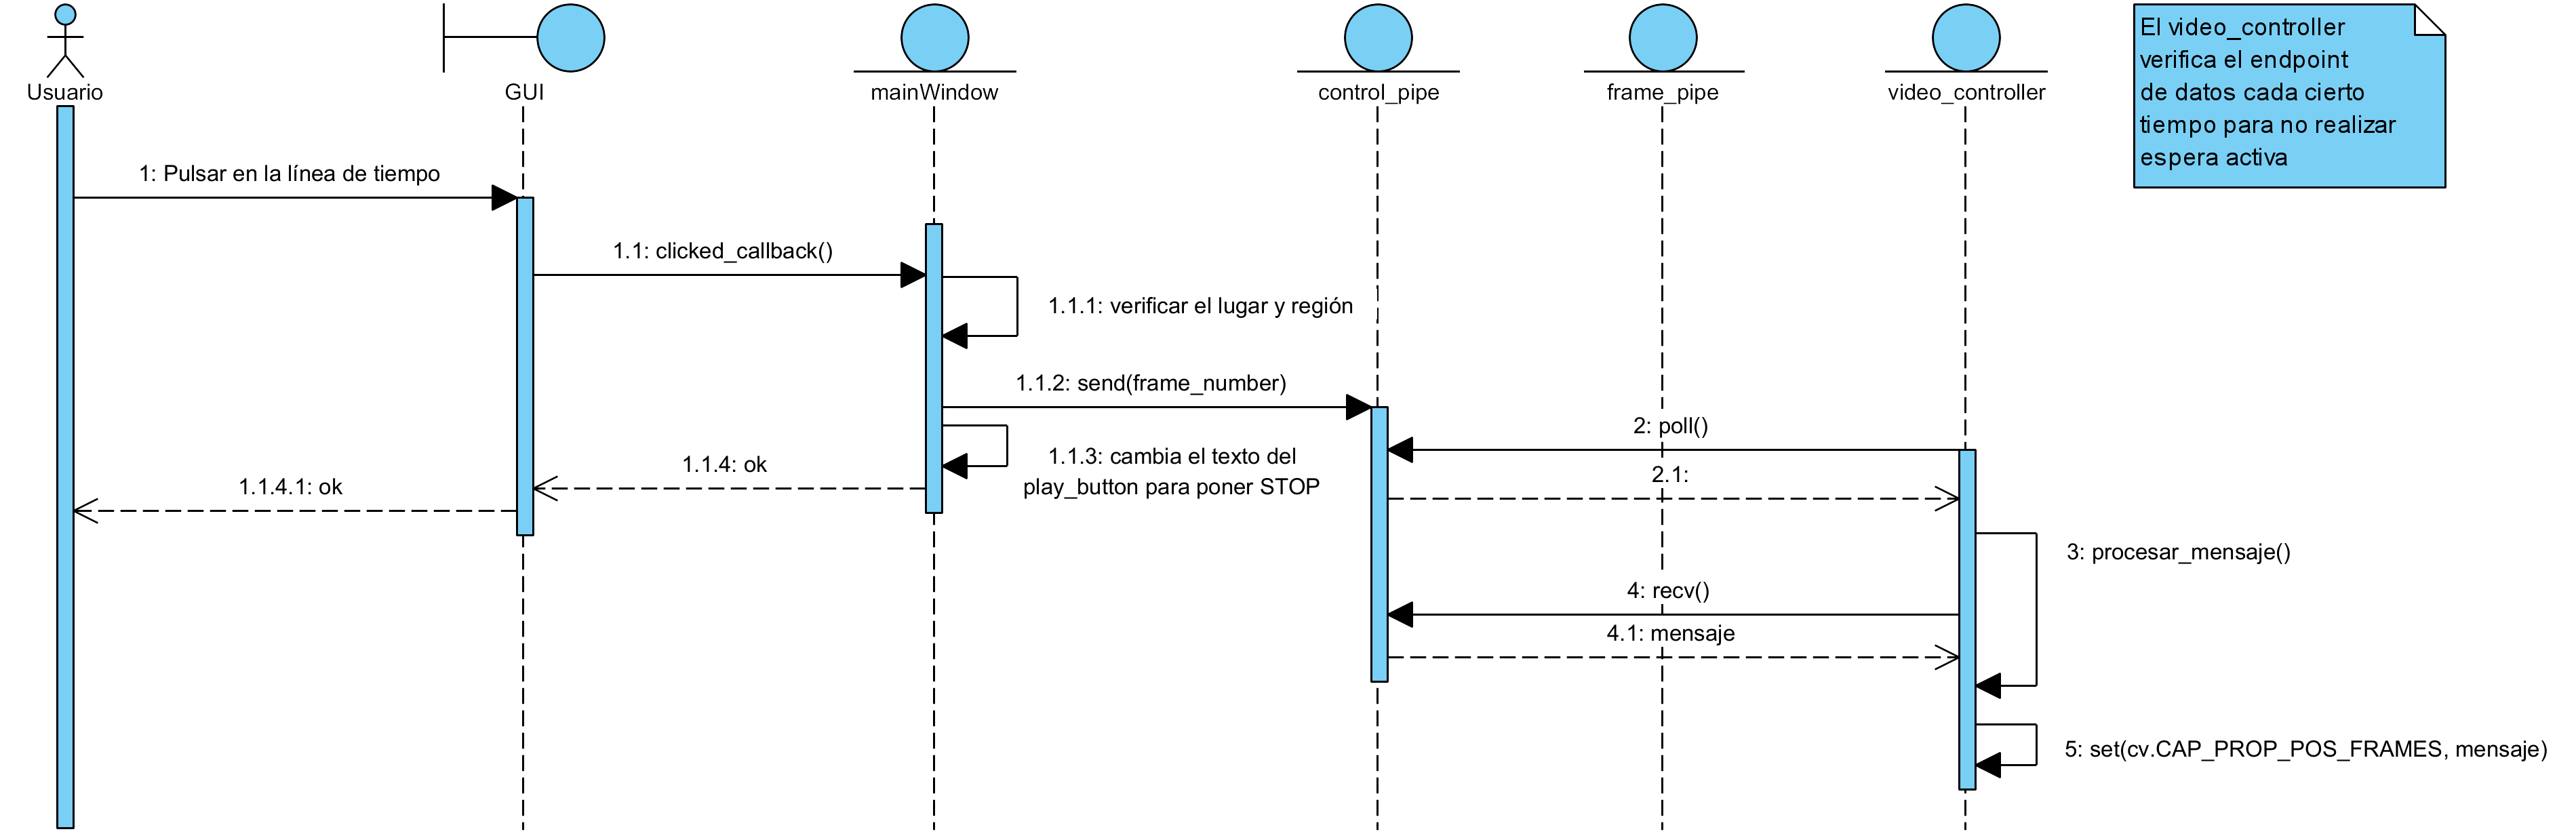
\includegraphics[width=\textwidth]{images/13/c/changeFrame.png}
    \caption{Diagrama de secuencia en el caso de uso de seleccionar algún fotograma en las líneas de tiempo}
\end{figure}